\documentclass[12pt,epsf,here,fleqn]{jreport}
\usepackage[dvipdfmx]{graphicx}
\usepackage[dvipdfmx]{color}
\usepackage{here}
\usepackage{fancybox}
\usepackage{psfrag}
\usepackage{amsmath,amssymb}
\usepackage{mediabb}
\usepackage{ulem}

\def\figurename{Fig.}
\def\tablename{Table}
\def\bibname{参考文献}

\setlength{\topmargin}{-1.0cm}
\setlength{\oddsidemargin}{1.0cm}
\setlength{\evensidemargin}{1.0mm}
\setlength{\textwidth}{15cm}
\setlength{\textheight}{23cm}
\setcounter{topnumber}{5}%    ページ上部の図表は 5 個まで
\def\topfraction{1.00}%       ページの上 1.00 まで図表で占めて可
\setcounter{bottomnumber}{5}% ページ下部の図表は 5 個まで
\def\bottomfraction{1.00}%    ページの下 1.00 まで図表で占めて可
\setcounter{totalnumber}{10}% ページあたりの図表は 10 個まで
\def\textfraction{0.04}%      ページうち本文が占める割合の下限
%        これを 0 にすると本文が 1 行だけのページが出来る
%        0.04 くらいにすると 1 行だけのページは防げる
%        0.1 くらいが良いかも知れない
\def\floatpagefraction{0.7}%  図表だけのページは少なくとも
                           %  これだけを図表が占める

\begin{document}%%%%%%%%ドキュメントの始まり
\baselineskip=0.8cm%%%%%タイトルの行間隔
%\documentclass[report, a4paper,11pt]{../thesis}
\usepackage[dvips]{graphicx}
\usepackage{ascmac} %枠で囲むやつら

%\renewcommand{\thesection}{\arabic{chapter}.\arabic{section}}
%\renewcommand{\thesubsection}{\arabic{chapter}.\arabic{section}.\arabic{subsection}}

\makeatletter       %参考文献を[1]から(1)へさらにciteを上付きへ
  \renewcommand{\@biblabel}[1]{(#1)}
  \DeclareRobustCommand\cite{\unskip
  \@ifnextchar[{\@tempswatrue\@citex}{\@tempswafalse\@citex[]}}
  \def\@cite#1#2{$\!^{\hbox{\scriptsize{(#1\if@tempswa , #2\fi})}}$}
  \def\@biblabel#1{#1)}
  \@addtoreset{figure}{chapter}
\makeatother

\addtolength{\oddsidemargin}{31truemm}
\addtolength{\textwidth}{-55truemm}
\setlength{\fullwidth}{\textwidth} 
%\addtolength{\topmargin}{-1truein}
\setlength{\headheight}{0pt}
\setlength{\headsep}{0pt}
\addtolength{\textheight}{20truemm}
\renewcommand{\baselinestretch}{1.2}
\newcommand{\figref}[1]{Fig:\ref{#1}}
\newcommand{\tableref}[1]{Table \ref{#1}}

\begin{document}

\pagestyle{empty}
%-----------------------------
%表紙
%-----------------------------
\newpage
\begin{center}
\vspace*{1cm}
{\Huge{○○年度}}\\
\vspace*{0.5cm}
{\Huge{卒業論文}}\\
\vspace*{2cm}
{\LARGE {○○○○○○の○○○○○○における\\○○○○○○の研究}}\\
\vspace*{5cm}
{\LARGE{神戸大学工学部情報知能工学科}}\\
\vspace*{1.0cm}
{\LARGE{神戸 太郎}}\\
\vspace*{1.5cm}
{\LARGE{\underline{指導教員\hspace{1.0cm}○○ ○○教授}}}\\
\vspace{3.0cm}
{\LARGE{2007年2月26日}}
\end{center}

\end{document}%%%%%%外タイトル
\newcommand{\hdate}[1]{\setcounter{page}{0}\begin{center}{\LARGE
#1\\}\vskip 20pt {\Huge 卒 業 論 文}\end{center}\vskip 40pt}

%題目が入ります
\newcommand{\htitle}[1]{
        \begin{center}
%                {\LARGE 題目}\\
                \vskip 16pt
                {\LARGE #1}\\
                \setlength{\unitlength}{1mm}
%               \vskip -20pt
%               \begin{picture}(100,10)(0,0)
%                       \put(0,0){\thicklines\line(1,0){100}}
%               \end{picture}
        \end{center}
        \vskip 40pt
}

\begin{titlepage}
\vspace*{2cm}
\hdate{2018年度}
\htitle{ティルトロータ型UAVにおける\\低速飛行特性の解析}

\hspace{8cm}
\begin{center}
\Large
神戸大学工学部情報知能工学科\\
\vskip 20pt
弓場~洋輝\\
\vskip 40pt
\underline{指導教員~~~~{\Large 玉置~久~~教授,浦久保~孝光~~准教授}}\\
%主査~~~~{\Large 玉置~久}\\
%副査~~~~{\Large 太田~能}\\
\vskip 20pt
%提出\\
2019年2月5日
\end{center}
\end{titlepage}
%%%%%%%内タイトル
\baselineskip=0.9cm%%%%%要旨の行間隔

\vspace*{13cm}
\begin{flushleft}
\hspace*{-9mm}
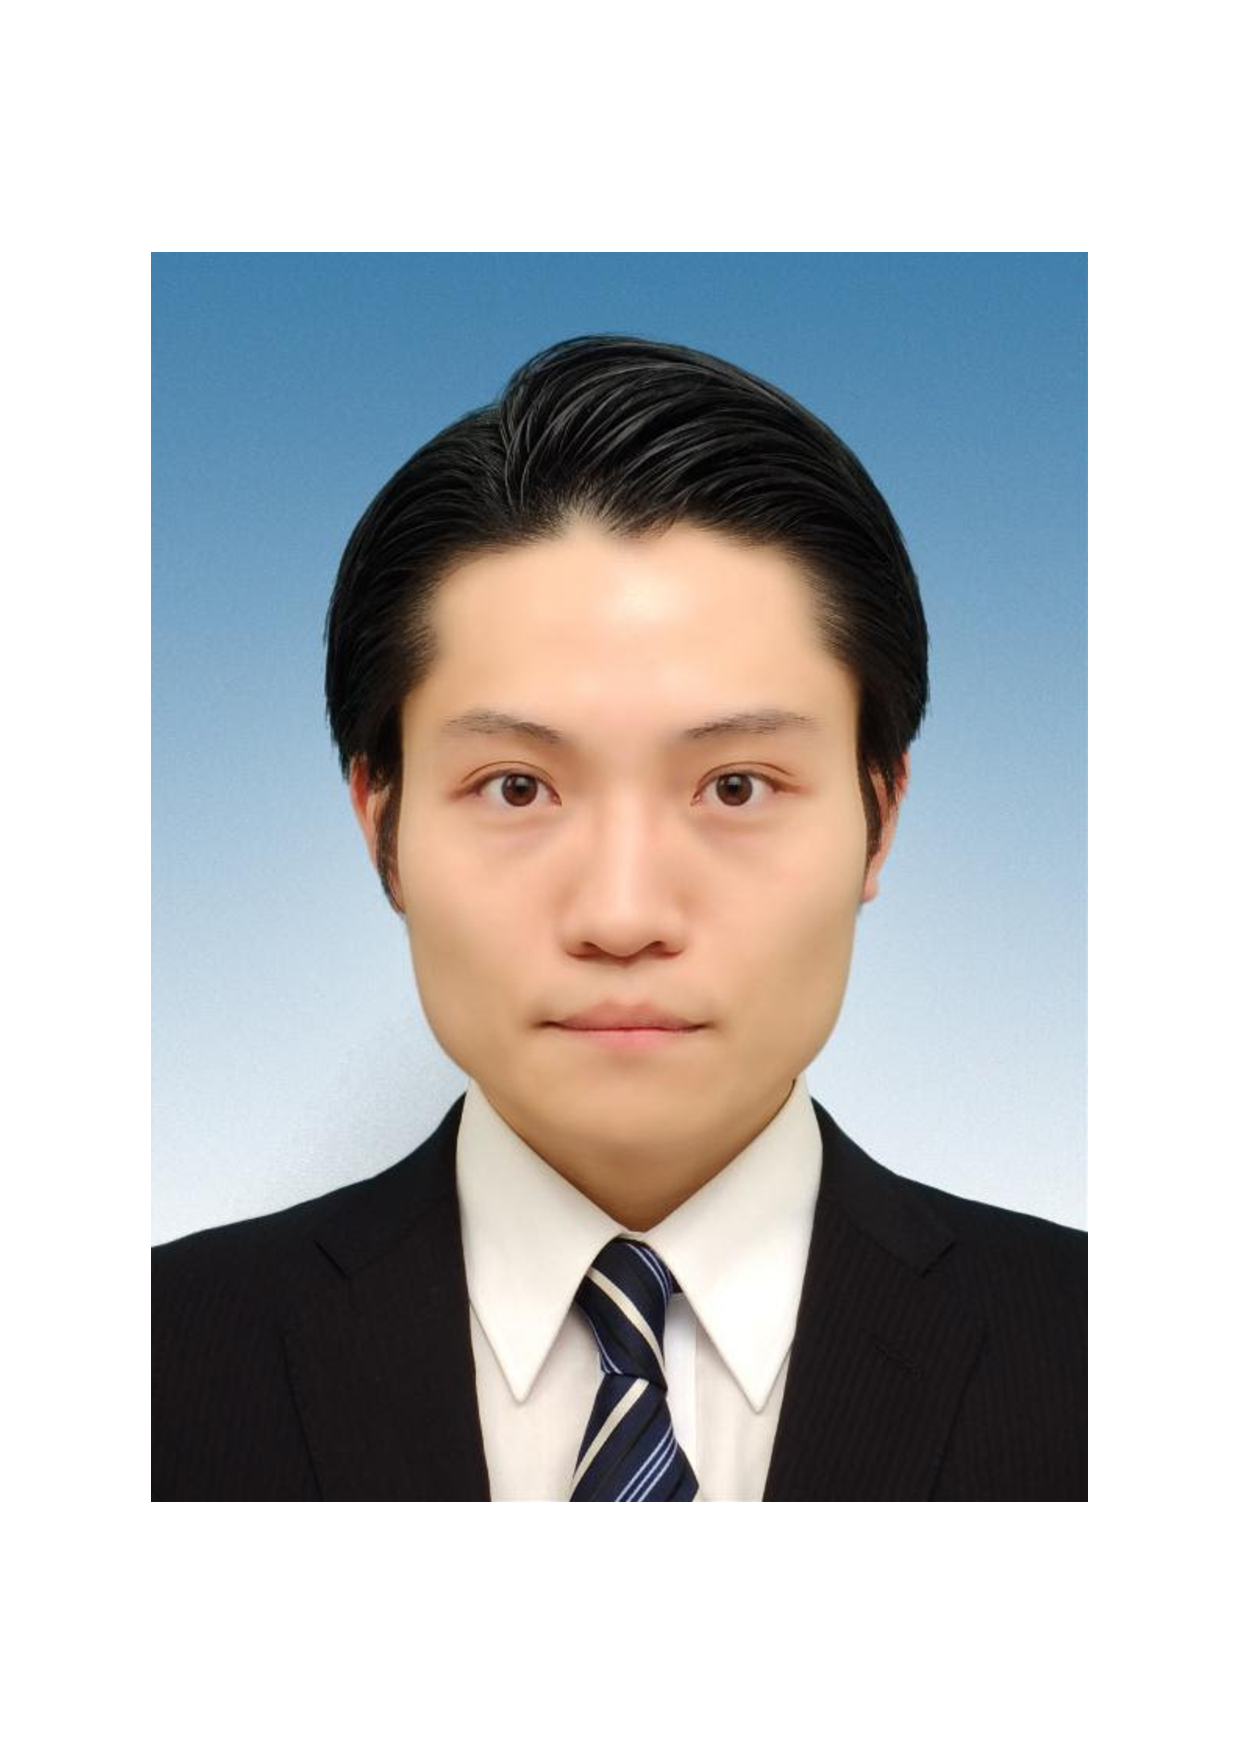
\includegraphics[height=8.3cm,width=6.0cm,clip]{z_figure_files/author.pdf}
\end{flushleft}
\vspace*{-5mm}
\hspace*{-9mm}
Copyright \copyright \, 2019, Hiroki Yuba

\thispagestyle{empty}%%%和文要旨ページ番号なし
% 要旨
%!TEX root = main.tex

\begin{titlepage}
%%% ページ番号つける?そのままだと番号がつきます.
%\thispagestyle{empty}
\begin{center}
{\LARGE \bf ティルトロータ型UAVにおける\\低速飛行特性の解析}
\\[0.5cm]
{\Large 弓場~洋輝}
\\[1.0cm]
{\LARGE \bf 要\vspace{36pt}   旨\\}
\end{center}

\indent

貯水施設や発電機がある放流路など様々な放流路から構成される水系の運用について,%
水系に存在する種々の制約を満たしつつも,効率的に水資源を利用する水系運用計画を%
作成することが肝要である.本研究では,効率的かつ実用的な水系運用計画の作成問題を%
対象として,数理計画モデルの一構成法を示すとともに,その妥当性について検討する.
\\
\indent
現状では,水系支援システムは種々の制約の充足などの機能が十分ではなく,%
実用的なものではない.そのため,運用計画の作成は%
現場の人手による対応に委ねられる部分が多くなっている.
本研究では,まず水系運用最適化問題を一般的に定義し,その定義に基づき,%
数理計画モデルとして定式化を行なう.
構成した数理計画モデルを現実的な水系を対象とした計算例を通して,モデルの妥当性について%
検討する.
\\
\indent
計算例より,制約を満たしつつ,水の効率的な運用がなされていることが確認できた.
この結果より提案モデルが一定の妥当性を有するものと考えられる.
水系運用計画を現実の運用に耐え得るものとするための,モデルのさらなる拡充・改良が今後の課題となる.

\end{titlepage}
%%%%%%%和文要旨
%\baselineskip=0.7cm%%%%目次の間隔狭い時ON
\baselineskip=0.9cm%%%%%目次の行間隔
\pagenumbering{roman}%%%目次のページ番号roman
\tableofcontents%%%%%%%%目次
\newpage%%%%%%%%%%%%%%%%改ページ
\baselineskip=0.7cm%%%%%本文の行間隔
\pagenumbering{arabic}%%本文のページ番号arabic
\setcounter{page}{1}%%%%本文のページ1から開始

% 第1章 序論
%!TEX root = main.tex

地震や津波などの自然現象による災害発生時,大規模で広範囲に及ぶ被災地での救助活動において,正確な情報収集を迅速かつ安全に行なうことが必要とされる.被災地では,建物の崩壊や地盤沈下などの理由による交通網の混乱で,地上における情報収集活動は困難となる.同時に,緊急を要する救援物資の運搬も難しくなる.

これらの課題に対し,地上状態の影響を受けない空の利用が有効であり,特に,無人航空機(Unmanned Aerial Veheicle, UAV)は有用である.UAVは,その名前のとおり操縦者を機体に搭乗しない航空機であり,大規模災害時に有人操縦者が行なうには危険な任務を遂行することが可能である.災害調査や空撮を行ない,荷物の積載能力や離着陸能力によっては,運搬利用も可能である.ただし物資運搬で利用する場合は,救助者の近くを飛行するため対人安全性も考慮しなければならない.

UAVは,飛行機のような形状の固定翼機と,ヘリコプタのようなロータ(回転翼)を持つ回転翼機に大きく分けられ,それぞれ異なる特徴を持つ.固定翼機は,速い巡航速度で飛行でき,推進効率も良いため長距離の飛行が可能であるが,一方で離着陸に滑走路が必要である.回転翼機は,垂直離着陸で,ホバリングも可能であるが,一方で固定翼機に比べて巡航速度が遅く,推進効率が悪い.

現在,災害発生時にUAVが利用される場合,それぞれの長所と短所を考慮し,災害状況や用途によって使い分けられている.しかし,大規模災害発生時においては,従来のUAVでは任務を効率的に遂行することができないため,より高い性能を持つUAVの開発が望まれる.

そこで我々は,固定翼機と回転翼機のそれぞれの長所をあわせ持つ,ティルトロータ機に着目した.ティルトロータ機とは,推力を発生させるメインロータを機体に対して鉛直方向から水平方向まで可動させることで,固定翼機モードと回転翼機モードを切り替えることができる航空機である.このようなティルトロータを有したUAVは,大規模災害発生時の情報収集に適した機体であると考えられる.本研究で使用するUAV(以下開発機体と表記)は,エアロセンス株式会社と共同で開発を行なったものである.軽量かつ剛性の高い,対人安全性を考慮した独自形状機構を持つ,ティルトロータを有した小型UAVである.

本研究では,開発機体を対象とし,特に回転翼機モード時の飛行特性解析を行なう.第2章では〜・・・

% 第2章
本章では,水系運用計画最適化問題について記述する.まず,水系運用計画最適化問題の概要に
ついて記述し,問題の基本要素と制約条件を述べる.

\section{問題の概要}
水系運用計画最適化問題とは,貯水施設と種々の放流路によって構成される水系において,%
各時間帯における放流路への放流量,特に,発電機が存在する放流路と貯水施設から水が溢れる%
こと(溢水)を防ぐために放流を行なう放流路への放流量を決定する問題である.
水系運用計画の作成には,貯水施設や各種放流路に存在する様々な制約を満たす必要がある.

\section{問題の記述}
水系運用計画最適化問題の基本要素,制約条件および評価指標を示す.
\subsection{基本要素}
	水系運用計画最適化問題における基本要素を列挙する.
	\subsubsection*{ダム} 
		ダムは放流路への水の放流を行なうものである.
		ダムには貯水機能を持つ通常のダムと持たないものがあり,貯水機能を持たないものを
		特に分流施設と呼ぶこととする.
		通常のダムは上流から流入する水を蓄え,任意の時間帯に放流を行なうことができるが,
		分流施設は上流から流入する水をそのまま下流へと流すこととなる.
	\subsubsection*{発電放流路}
		発電放流路は発電機が存在する放流路である.
		この放流路に放流がなされることによって,発電が行なわれる.
	\subsubsection*{ゲート放流路}
		ダムからの溢水を防ぐための放流を行なう放流路である.
	\subsubsection*{バイパス放流路}
		主に周囲の環境の維持を目的として放流が行われる放流路である.	
	\subsubsection*{スイッチ放流路}
		特定の発電機群の運転状況に応じて放流が行なわれる放流路である.
		発電機群が運転していれば放流が行なわれる放流路と
		停止していれば放流が行なわれる放流路の2つが存在する.
	\subsubsection*{特別放流路}
		以上の放流路のいずれにも属さず,発電・ゲート放流量を決定することにより,
		放流量が定まる放流路である.
\subsection{制約条件}
	水系運用計画最適化問題における制約条件を要素ごとにまとめる.
	\subsubsection*{ダム} 
		\begin{itemize}
			\item 貯水量制約 \\
			 ダムの貯水量が許容範囲内になければならない.
			\item 最終貯水量制約 \\
			 ダムの貯水量の最終値が許容範囲内になければならない.
		\end{itemize}	
	\subsubsection*{発電放流路}
		\begin{itemize}
			\item 水量制約 \\
			 発電機の運転時には使用水量が許容範囲内になければならない.
			\item 電水比制約 \\
			 電水比により,発電機の使用水量と発電電力量が規定される.
			\item 計画運転・停止制約 \\
			 計画運転・停止期間において発電機は運転,%
			または停止状態になければならない.
			\item 短時間運転・停止制約 \\
			 短時間の間に発電機の運転と停止を切り替えるのは望ましくなく,
			停止している発電機を起動すると,一定時間は運転を継続する必要がある.
			また,発電機を停止すると,起動には一定時間間隔を空ける必要がある.
			\item ALL制約 \\
			 周囲の環境への影響を抑えるため,%
			発電所(特定の発電機の組)に使用する水量は%
			段階的に上昇させなければならない.
			\item 夜間出力増制約 \\
			 発電機の出力増加には騒音が伴うため,%
			夜間の時間帯では発電機の出力を増加させてはならない.
		\end{itemize}
	\subsubsection*{スイッチ放流路}
		\begin{itemize}
			\item 分流制約 \\
			 スイッチ放流路は特定の発電機群の運転状況によって,%
			放流を行なうかどうかが決まる.発電機群が運転しているときに放流を行なう
			放流路と停止しているときに放流を行なう放流路の2つがある.
		\end{itemize}	
	\subsubsection*{ゲート放流路,スイッチ放流路,特別放流路}
		\begin{itemize}
			\item 放流量制約 \\
			 すべての放流路について,放流量は許容範囲内になければならない.
		\end{itemize}
	
	\subsection{評価指標}
		時間帯ごとの発電価値の総和最大化とゲート放流量の総和最小化を評価指標とする.
		
\section{まとめ}
本章では,水系運用計画最適化問題の概要を述べ,問題の基本要素,制約条件ならびに評価指標%
について記述した.次章では,本章での記述に基づいた数理計画モデルを示す.
% 第3章
%!TEX root = main.tex

本章では,機体を単一の剛体とみなしたときの6自由度(3軸方向,3軸まわり回転)非線形運動方程式,および3つの姿勢角(オイラー角)の微分方程式による,計9次の非線形微分方程式を記述し,特に縦運動(前後,上下,機首の上下回転運動)にのみ着目し,飛行モデルを設定する.さらに,微小運動を仮定した非線形モデルの線形化を行なう.最後に,機体まわりに働く空気力のモデルの設定について述べる.

%%%%%%%%%%%%%%%%%%%%%%
\section{座標系の導入}
%%%%%%%%%%%%%%%%%%%%%%

\ref{}に示すように,機体に固定した回転座標系$a^{(B)}-x_B,y_B,z_B$(機体座標系)を導入する.また,機体の姿勢を定義するため,\ref{}に示すように,地球に固定した$a^{(E)}-x_E,y_E,z_E$(地球固定座標系)を導入する.

機体姿勢は,姿勢角$\psi,\theta,\phi$によって表し,それぞれヨー角,ピッチ角,ロール角である.これらはオイラー角とよばれ,この順序で機体を回転させることにより,座標系の変換を行なう.

\subsection{座標系の変換}

例えば,$a^{(E)}$から$a^{(B)}$への座標変換行列を$A^{(B,E)}$と書くとすると
\begin{equation}
  \left[
    \begin{array}{ccc}
      x \\
      y \\
      z
    \end{array}
  \right]_B =
  A^{(B,E)}
  \left[
    \begin{array}{ccc}
      x \\
      y \\
      z
    \end{array}
  \right]_E
\end{equation}
となり
\begin{equation}
  \begin{split}
    A^{(B,E)} &=
    \left[
      \begin{array}{ccc}
        1 & 0 & 0 \\
        0 & c\phi & s\phi \\
        0 & -s\phi & c\phi
      \end{array}
    \right]
    \left[
      \begin{array}{ccc}
        c\theta & 0 & -s\theta \\
        0 & 1 & 0 \\
        s\theta & 0 & c\theta
      \end{array}
    \right]
    \left[
      \begin{array}{ccc}
        c\psi & s\psi & 0 \\
        -s\psi & c\psi & 0 \\
        0 & 0 & 1
      \end{array}
    \right] \\
    &=
    \left[
  	\begin{array}{ccc}
    	c\theta c\psi & c\theta s\psi & -s\theta \\
    	s\phi s\theta c\psi - c\phi s\psi & s\phi s\theta s\psi + c\phi c\psi & s\phi c\theta \\
    	c\theta s\theta c\psi + s\phi s\psi & c\phi s\theta s\psi - s\phi c\psi & c\phi c\theta
  	\end{array}
  	\right]
  \end{split}
\end{equation}
のように表される.簡略のため,$\sin* = s*$,$\cos* = c*$と表記している.

また,$A^{(B,E)}$は直交行列であり,逆行列は転置行列に等しいため
\begin{equation}
  A^{(E,B)} =
  \left[
  \begin{array}{ccc}
    c\theta c\psi & s\phi s\theta c\psi - c\phi s\psi & c\theta s\theta c\psi + s\phi s\psi \\
    c\theta s\psi & s\phi s\theta s\psi + c\phi c\psi & c\phi s\theta s\psi - s\phi c\psi \\
    -s\theta & s\phi c\theta & c\phi c\theta
  \end{array}
  \right]
\end{equation}
となる.

\subsection{オイラー角の微分方程式}

オイラー角と機体角速度の関係は
\begin{equation}
  \left[
  \begin{array}{ccc}
    \dot{\phi} \\
    \dot{\theta} \\
    \dot{\psi}
  \end{array}
  \right]
   =
  \left[
  \begin{array}{ccc}
    1 & \sin\phi\tan\theta & \cos\phi\tan\theta \\
    0 & \cos\phi & -\sin\phi \\
    0 & \frac{\sin\phi}{\cos\theta} & \frac{\cos\phi}{\cos\theta}
  \end{array}
  \right]
  \left[
  \begin{array}{ccc}
    p \\
    q \\
    r
  \end{array}
  \right]
\end{equation}
となり,これはオイラー角のキネマティクス方程式とよばれる.ここで,$\dot{\phi},\dot{\theta},\dot{\psi}$はそれぞれ姿勢角の時間微分であり,$p,q,r$はそれぞれ機体座標系における角速度の$x,y,z$成分である.

%%%%%%%%%%%%%%%%%%%%%%
\section{非線形モデル}
%%%%%%%%%%%%%%%%%%%%%%

並進運動と回転運動について,それぞれ運動方程式を記述する.その後,回転翼機モードでの低速飛行における縦運動の運動方程式についてまとめ,機体の非線形モデルとして設定する.

\subsection{非線形並進運動方程式}

機体座標系で表した並進運動方程式は,機体重量を$m$として
\begin{equation}
  \left[
  \begin{array}{ccc}
    \dot{u} \\
    \dot{v} \\
    \dot{w}
  \end{array}
  \right]
   =
  \left[
  \begin{array}{rrr}
    0 & r & -q \\
    -r & 0 & p \\
    q & -p & 0
  \end{array}
  \right]
  \left[
  \begin{array}{ccc}
    u \\
    v \\
    w
  \end{array}
  \right] + \dfrac{1}{m}
  \left[
  \begin{array}{ccc}
    F_x \\
    F_y \\
    F_z
  \end{array}
  \right]
  \label{mot_eq}
\end{equation}
where
\begin{equation*}
  \mbox{\boldmath $V$} =
  \left[
  \begin{array}{c}
    u \quad v \quad w
  \end{array}
  \right]^{\mathrm{T}} :
  \mbox{機体の速度}
\end{equation*}
\begin{equation*}
  \mbox{\boldmath $F$} =
  \left[
  \begin{array}{c}
    F_x \quad F_y \quad F_z
  \end{array}
  \right]^{\mathrm{T}} :
  \mbox{機体に働く力}
\end{equation*}
となる.式(\ref{mot_eq})の右辺第2項の力は,重力,空気力,ロータ推力に分けて
\begin{equation}
    \mbox{\boldmath $F$} = \mbox{\boldmath $F_g$} + \mbox{\boldmath $F_a$} + \mbox{\boldmath $F_t$}
\end{equation}
where
\begin{align*}
  \mbox{\boldmath $F_g$} =
  \left[
  \begin{array}{c}
    X_g \quad Y_g \quad Z_g
  \end{array}
  \right]^{\mathrm{T}},
  \mbox{\boldmath $F_a$} =
  \left[
  \begin{array}{c}
    X_a \quad Y_a \quad Z_a
  \end{array}
  \right]^{\mathrm{T}},
  \mbox{\boldmath $F_t$} =
  \left[
  \begin{array}{c}
    X_t \quad Y_t \quad Z_t
  \end{array}
  \right]^{\mathrm{T}}
\end{align*}
と書ける.ここで重力について
\begin{equation}
  \mbox{\boldmath $F_g$} \triangleq
  \left[
  \begin{array}{ccc}
    X_g \\
    Y_g \\
    Z_g
  \end{array}
  \right] =
  A^{(B,E)}
  \left[
  \begin{array}{ccc}
    0 \\
    0 \\
    mg
  \end{array}
  \right] = mg
  \left[
  \begin{array}{ccc}
    -\sin\theta \\
    \sin\phi\cos\theta \\
    \cos\phi\cos\theta
  \end{array}
  \right]
\end{equation}
である.またロータ推力について,$y$軸方向の力$Y_t=0$であるから,ティルト角を$\gamma$,メインロータ推力を$T_m$,右左サブロータ推力を$T_r$,機首サブロータ推力を$T_f$とすれば次のようになる.
\begin{equation}
  \mbox{\boldmath $F_t$} \triangleq
  \left[
    \begin{array}{ccc}
      X_t \\
      Y_t \\
      Z_t
    \end{array}
  \right] =
  \left[
    \begin{array}{ccc}
      -\cos\gamma & 0 & \sin\gamma \\
      0 & 0 & 0 \\
      -\sin\gamma & 0 & -\cos\gamma
    \end{array}
  \right]
  \left[
    \begin{array}{ccc}
      0 \\
      0 \\
      T_m
    \end{array}
  \right] -
  \left[
    \begin{array}{ccc}
      0 \\
      0 \\
      T_r + T_f
    \end{array}
  \right]
\end{equation}

空気力項については,\ref{}で詳しく述べる.

% \begin{equation}
%   \left[
%   \begin{array}{ccc}
%     \dot{u} \\
%     \dot{v} \\
%     \dot{w}
%   \end{array}
%   \right]
%    =
%   \left[
%   \begin{array}{rrr}
%     0 & r & -q \\
%     -r & 0 & p \\
%     q & -p & 0
%   \end{array}
%   \right]
%   \left[
%   \begin{array}{ccc}
%     u \\
%     v \\
%     w
%   \end{array}
%   \right] + g
%   \left[
%   \begin{array}{ccc}
%     -\sin\theta \\
%     \sin\phi\cos\theta \\
%     \cos\phi\cos\theta
%   \end{array}
%   \right] + \dfrac{1}{m}
%   \left[
%   \begin{array}{ccc}
%     X_a + X_t \\
%     Y_a + Y_t \\
%     Z_a + Z_t
%   \end{array}
%   \right]
% \end{equation}

\subsection{非線形回転運動方程式}

次に,回転の運動について考える.本研究で開発した機体は,機体座標系における$x$軸と$z$軸で張られる面に対し面対称であるため,慣性乗積を0とすると,慣性行列は次のようになる.
\begin{equation}
  I =
  \left[
  \begin{array}{ccc}
    I_{xx} & 0 & -I_{xz} \\
    0 & I_{yy} & 0 \\
    -I_{xz} & 0 & I_{zz}
  \end{array}
  \right]
\end{equation}
このとき,機体の回転運動方程式は
\begin{equation}
I\left[
  \begin{array}{ccc}
    \dot{p} \\
    \dot{q} \\
    \dot{r}
  \end{array}
  \right] =
  \left[
  \begin{array}{rrr}
    0 & r & -q \\
    -r & 0 & p \\
    q & -p & 0
  \end{array}
  \right]
  I
  \left[
  \begin{array}{ccc}
    p \\
    q \\
    r
  \end{array}
  \right] +
  \left[
  \begin{array}{ccc}
    L \\
    M \\
    N
  \end{array}
  \right]
  \label{roll_eq}
\end{equation}
where
\begin{equation*}
  \mbox{\boldmath $M$} =
  \left[
  \begin{array}{c}
    L \quad M \quad N
  \end{array}
  \right]^{\mathrm{T}} :
  \mbox{各機体軸まわりのモーメント}
\end{equation*}
となる.式(\ref{roll_eq})の右辺第2項のモーメントは,重力,空気力,ロータ推力それぞれによるモーメントに分けて
\begin{equation}
    \mbox{\boldmath $M$} = \mbox{\boldmath $M_g$} + \mbox{\boldmath $M_a$} + \mbox{\boldmath $M_t$}
\end{equation}
where
\begin{align*}
  \mbox{\boldmath $M_g$} =
  \left[
  \begin{array}{c}
    L_g \quad M_g \quad N_g
  \end{array}
  \right]^{\mathrm{T}},
  \mbox{\boldmath $M_a$} =
  \left[
  \begin{array}{c}
    L_a \quad M_a \quad N_a
  \end{array}
  \right]^{\mathrm{T}},
  \mbox{\boldmath $M_t$} =
  \left[
  \begin{array}{c}
    L_t \quad M_t \quad N_t
  \end{array}
  \right]^{\mathrm{T}}
\end{align*}
と書ける.ここで重力について,機体軸原点から重心までの距離ベクトルを\mbox{\boldmath $R_G$}とすれば
\begin{equation}
  \begin{split}
    \mbox{\boldmath $M_g$} \triangleq
    \left[
    \begin{array}{ccc}
      L_g \\
      M_g \\
      N_g
    \end{array}
    \right] =
    \mbox{\boldmath $R_G$} \times
    m\mbox{\boldmath $g$} &=
    \left[
    \begin{array}{ccc}
      R_{G_x} \\
      0 \\
      R_{G_z}
    \end{array}
    \right] \times
    A^{(B,E)}
    \left[
    \begin{array}{ccc}
      0 \\
      0 \\
      mg
    \end{array}
    \right] \\
    &= mg
    \left[
    \begin{array}{ccc}
      R_{G_z}\cos\theta\sin\phi \\
      -R_{G_z}\sin\theta - R_{G_x}\cos\theta\cos\phi \\
      R_{G_x}\cos\theta\sin\phi
    \end{array}
    \right]
  \end{split}
\end{equation}
である.また,ロータ推力によるモーメントは,\ref{}によるとまだ未解明な点も多いため,本研究で扱う縦運動に関係するピッチングモーメント$M_t$のみ記載することにする.機体軸原点から各ロータまでの距離を\ref{}のように定めると
\begin{equation}
  M_t = -l_m T_m \cos\gamma + l_f T_f - l_{r_y} T_r
\end{equation}

空気力項については,\ref{}で詳しく述べる.

%%%%%%%%%%%%%%%%%%%%%%
\section{空気力モデル}
%%%%%%%%%%%%%%%%%%%%%%



%%%%%%%%%%%%%%%%%%%%
\section{線形モデル}
%%%%%%%%%%%%%%%%%%%%

% 第4章
%!TEX root = main.tex
本章では,に示した数理計画モデルによる,
実際の水系に準ずる例題を用いた計算例を示し,%
構築したモデルの妥当性について検討する.
なお,求解には数理計画パッケージCPLEX12\cite{cplex}を用いた.
%%%%%%%%%%
\section{問題設定}
%%%%%%%%%%

計画期間を24時間,時間帯幅を10分とした問題を考える.
Fig. \ref{fig:watersystem}およびFig. \ref{fig:value}に対象とする水系と%
各時間帯における発電価値を示す.
発電価値は需要が多い時間帯に高くなることから,%
今回は需要曲線を元に作成したものを使用した.
Fig. \ref{fig:watersystem}における,台形,長方形および円形のシンボルがそれぞれダム,%
分流施設,発電放流路を表している.\\
また,Tables. \ref{storage}〜\ref{storage2}に水系の基本情報などのパラメータの設定値を示す.
\indent
問題の設定として,以下を想定する.
\begin{itemize}
	\item
	スイッチ放流路$\rm Y_{5,6},\rm Y_{5,7}$は%
	発電機$\rm G_{810}$系と対応しており,$\rm G_{810}$系の運転時には$\rm Y_{5,7}$に%
	放流を行ない,停止時には$\rm Y_{5,6}$に放流を行なう.
	\item
	目的関数については$w=100,000$とし,ゲート放流に対するペナルティが%
	大きくなるようにすることで,ゲート放流量を可能な限り抑える.
	\item
	短時間運転・停止制約における連続運転・停止期間を%
	1時間として設定する.
	\item
	20時から6時を夜間とする.
	\item
	計画運転・停止期間は設定しない.
	\item
	$\rm D_{2}$については,そこからの発電放流量は%
	すべて予め計画されているものとする.
	\item
	バイパス放流量および渓流量はそれぞれの放流路やダムで常に一定とし,
	1時間帯当たりの水量をTable. \ref{bypass}および\ref{stream}に示す.
\end{itemize}

\begin{figure}[H]
  \centering
  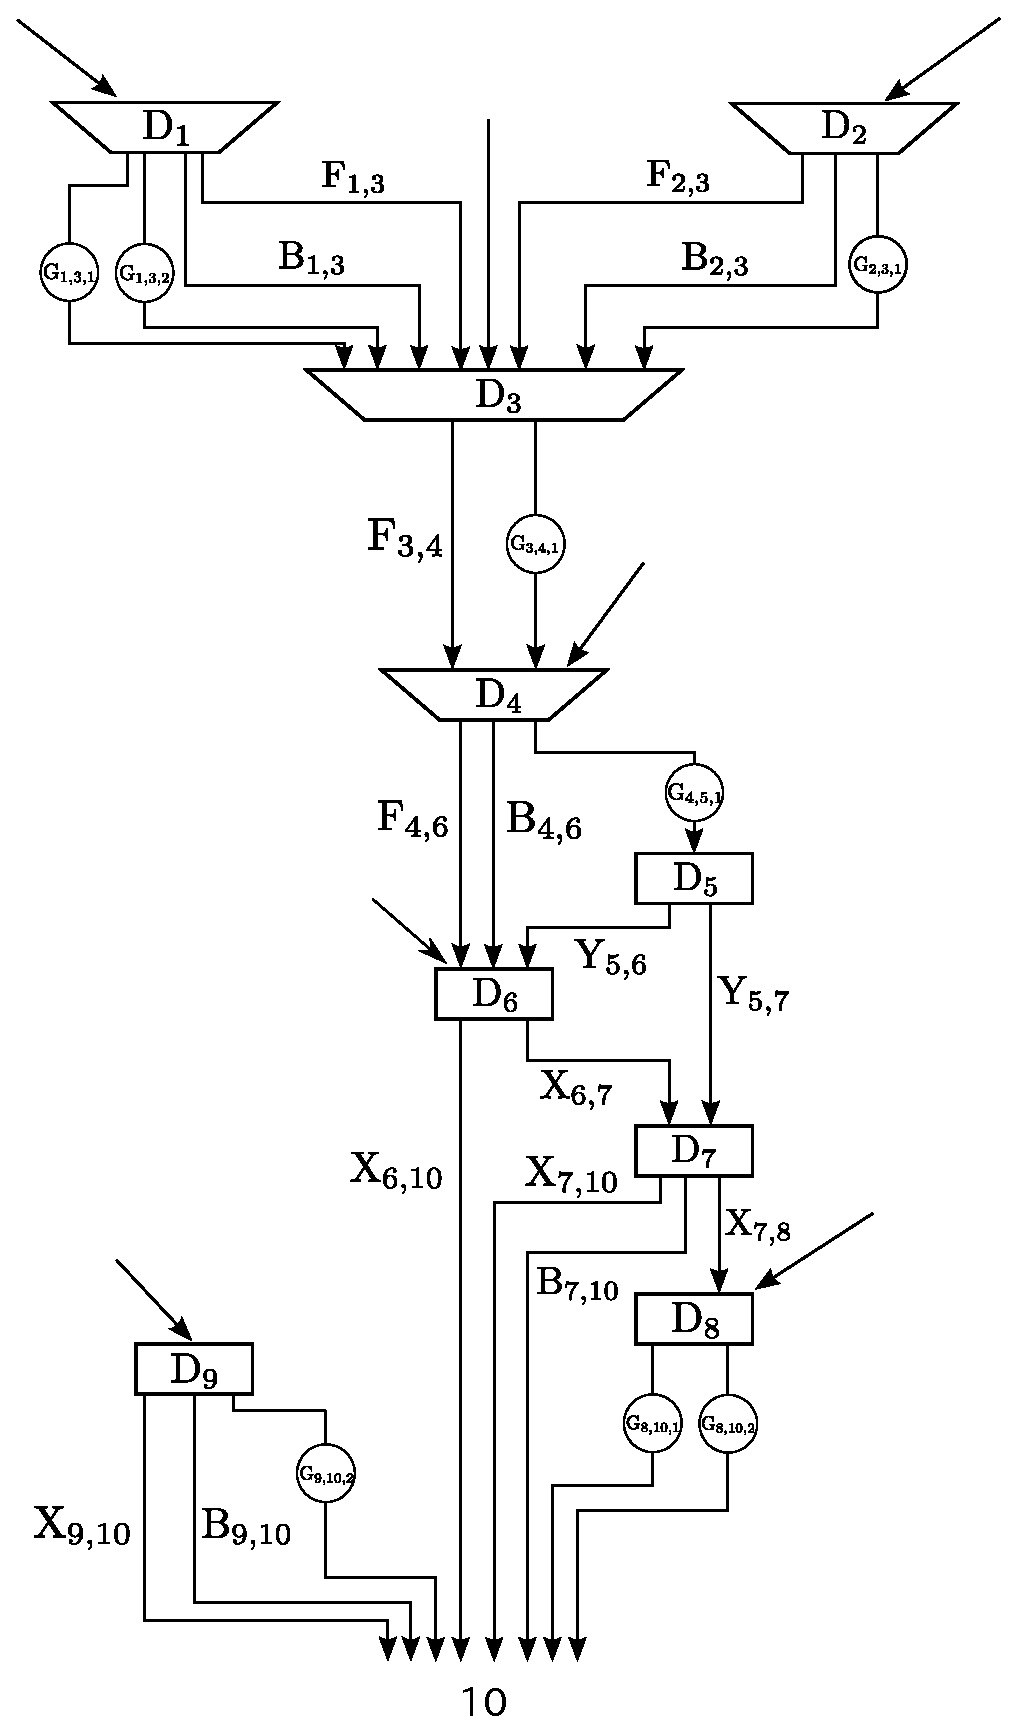
\includegraphics[width=0.85\linewidth]{fig/JinzuRev3.eps}
  \caption{Water system}
  \label{fig:watersystem}
\end{figure}

\begin{figure}[H]
  \centering
  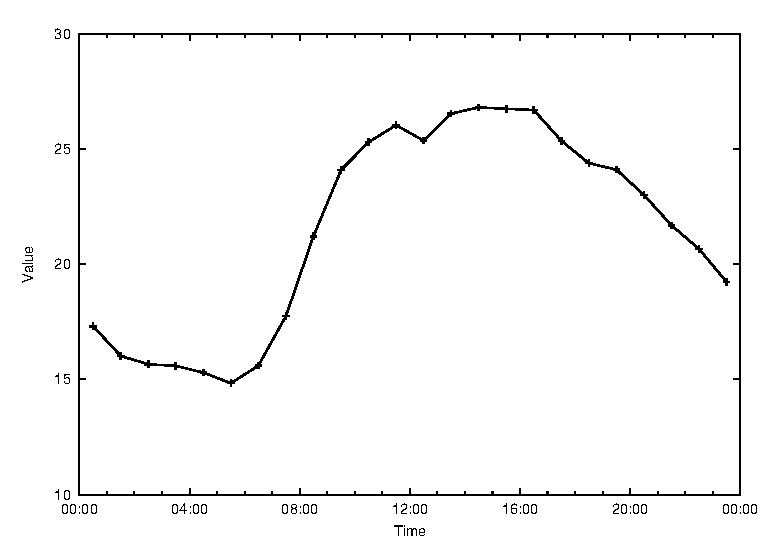
\includegraphics[width=0.9\linewidth]{fig/val.eps}
  \caption{Value of electric energy}
  \label{fig:value}
\end{figure}

\begin{table}[htbp]
\begin{center}
\caption{Storage of dam}
\label{storage}
\begin{tabular}{llllll}
\hline
Number & 1 & 2 & 3 & 4\\
\hline \hline
$s^{\rm Min}$ & 142,707 & 0 & 625,409 & 1,152,112 & \\
$s^{\rm Max}$ & 553,791 & 117,935,420 & 1,370,298 & 2,698,099\\
\hline
\end{tabular}
\label{storage}
\end{center}
\end{table}

\begin{table}[htbp]
\label{table:7}
\begin{center}
\caption{Generator Data}
\vspace*{-5mm}
\begin{tabular}{ccccccccc}
\hline
Generator Number & 131 & 132 & 231 & 341 & 451 & 8101 & 8102 & 9101 \\ \hline \hline
$q^{\rm G,Max}$[$\rm{m^3}$] & 20640 & 20640 & 39000 & 22200 & 23640 & 13080 & 13080 & 3000 \\
$q^{\rm G,Min}$[$\rm{m^3}$] & 5400 & 5400 & 8520 & 7041 & 8006 & 1344 & 1344 & 124\\
$\alpha$[$\rm{kWh/m^3}$] & 0.0788 & 0.0786 & 0.6069 & 0.0583 & 0.1680 & 0.3250 & 0.3222 & 0.6888\\
$\tau^{\rm G,Up}$ & 0 & 0 & 0 & 0 & 0 & 0 & 0  & 0 \\
$\tau^{\rm G,Down}$ & 2 & 2 & 1 & 2 & 2 & 0 & 0  & 0 \\
\hline
\end{tabular}
\end{center}
\end{table}

\begin{table}[htbp]
\begin{center}
\caption{Gate waterway Data}
\label{gate}
\begin{tabular}{ccccccc}
\hline
Number &13 & 23 & 34 & 46 \\ \hline \hline
$q^{\rm F,Max}$[$\rm {10^{-4} \cdot m^3}$] & 138 & 102 & 174 & 180 \\
$\tau^{\rm F}$ & 0 & 0 & 0 & 0 \\
\hline
\end{tabular}
\end{center}
\end{table}

\begin{table}[htbp]
\begin{center}
\caption{Special waterway Data}
\label{way}
\begin{tabular}{llllll}
\hline
Number & 67 & 78 & 710 & 610 & 910\\ \hline
$q^{\rm X,Max}$[$ \rm {m^3}$] & 24,000 & 24,000 & 24,000 & 2,100,000 & 300,000 \\
$\tau^{\rm X}$& 0 & 0 & 0 & 0 & 0 \\
\hline
\end{tabular}
\end{center}
\end{table}

\begin{table}[htbp]
\begin{center}
\caption{Switch waterway Data}
\label{switch}
\label{table:way2}
\begin{tabular}{ccc}
\hline
Number & 56 & 57 \\ \hline
$q^{\rm Y,Max}$[$ \rm {m^3}$] & 23,700 & 23,700 \\
\hline
\end{tabular}
\end{center}
\end{table}

\begin{table}[htbp]
\begin{center}
\caption{First and last storage of dam}
\label{storage2}
\begin{tabular}{llllll}
\hline
Number & 1 & 2 & 3 & 4\\
\hline \hline
$s^{\rm Last,Min}$ & 409,419 & 26,340,350 & 1,156,164 & 2,247,878\\
first & 409,419 & 73,786,986 & 1,156,164 & 2,247,878 \\
$s^{\rm Last,Max}$ & 409,419 & 117,935,420 & 1,156,164 & 2,247,878\\
\hline
\end{tabular}
\label{storage}
\end{center}
\end{table}

\begin{table}[htbp]
\begin{center}
\caption{Bypass discharge}
\label{bypass}
\begin{tabular}{ccccc}
\hline
$\rm B_{13}$ & $\rm B_{23}$ & $\rm B_{46}$ & $\rm B_{710}$ & $\rm B_{910}$ \\
\hline
\hline
0 & 360 & 0 & 3,339 & 0\\
\hline
\end{tabular}
\end{center}
\end{table}

\begin{table}[htbp]
\begin{center}
\caption{Mountain stream}
\label{stream}
\begin{tabular}{ccccccccc}
\hline
1 & 2 & 3 & 4 & 5 & 6 & 7 & 8 & 9\\
\hline
\hline
3,000 & 3,000 & 1,200 & 3,000 & 0 & 0 & 0 & 0 & 1,440\\
\hline
\end{tabular}
\end{center}
\end{table}


\newpage
%%%%%%%%%%%%%%%%
\section{計算結果および考察}
%%%%%%%%%%%%%%%%

%目的関数値:47689359
%計算時間:31.95[sec]

Figs. \ref{fig:d1}〜\ref{fig:d9}に,結果として得られた各ダムの貯水量の推移と
そのダムからの発電放流量を示す%
(Figs. \ref{fig:d1}〜\ref{fig:d4}においては上下限貯水量も示している).
ただし,$\rm D_{8}$および$\rm D_{9}$は分流施設であり,貯水機能を持たないので,%
$\rm G_{8,10,1}$,$\rm G_{8,10,2}$,$\rm G_{9,10,1}$への%
発電放流量のみFig. \ref{fig:d8}およびFig. \ref{fig:d9}に示している.

Figs. \ref{fig:d1}〜\ref{fig:d8}の結果より,いずれの発電放流路においても,%
発電価値の高い時間帯での可能な限りの放流が行なわれる結果となっていることが
確認できる($\rm D_{9}$は渓流のみが流れ込む分流施設であるため,%
常に一定の発電放流を行なっている(Fig. \ref{fig:d9})).
また,貯水量および放流量の上下限等の制約も満たされていることがわかる.
これらより,本研究で構成した数理計画モデルは妥当なものであると考えられる.

\begin{figure}[H]
  \centering
  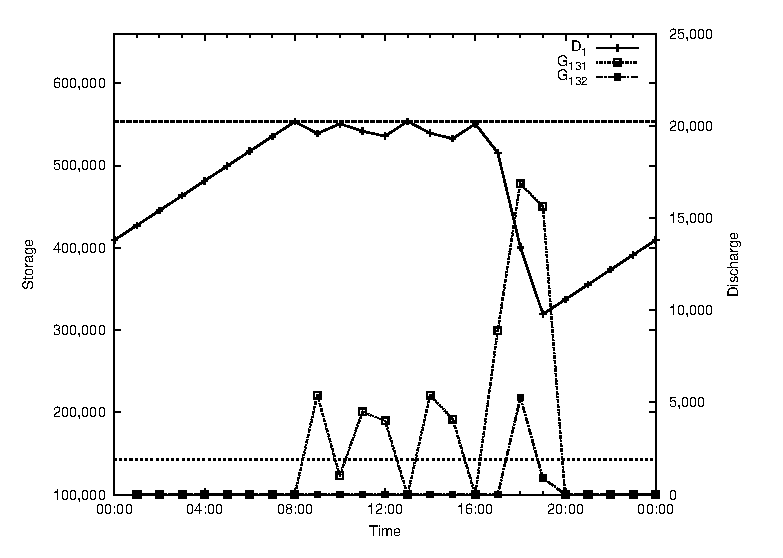
\includegraphics[width=0.9\linewidth]{fig/d1.eps}
  \caption{Storage in $\rm D_{1}$ and Generation Discharge}
  \label{fig:d1}
\end{figure}

\begin{figure}[H]
  \centering
  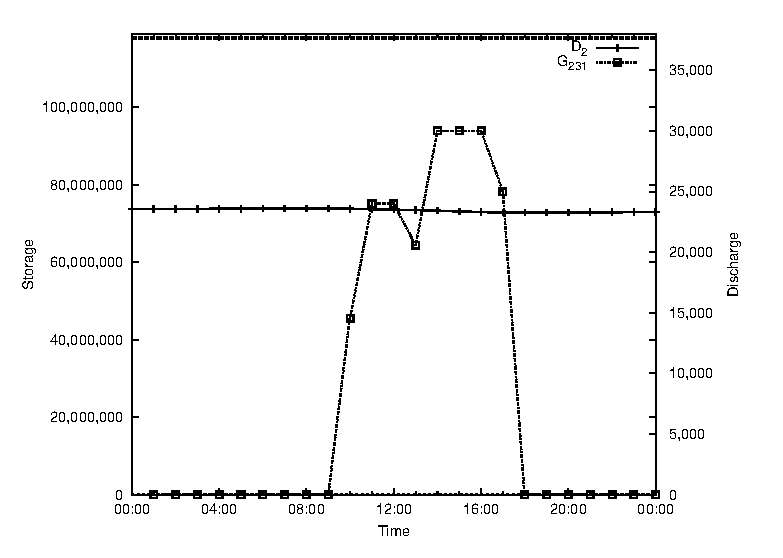
\includegraphics[width=0.9\linewidth]{fig/d2.eps}
  \caption{Storage in $\rm D_{2}$ and Generation Discharge }
  \label{fig:d2}
\end{figure}

\begin{figure}[H]
  \centering
  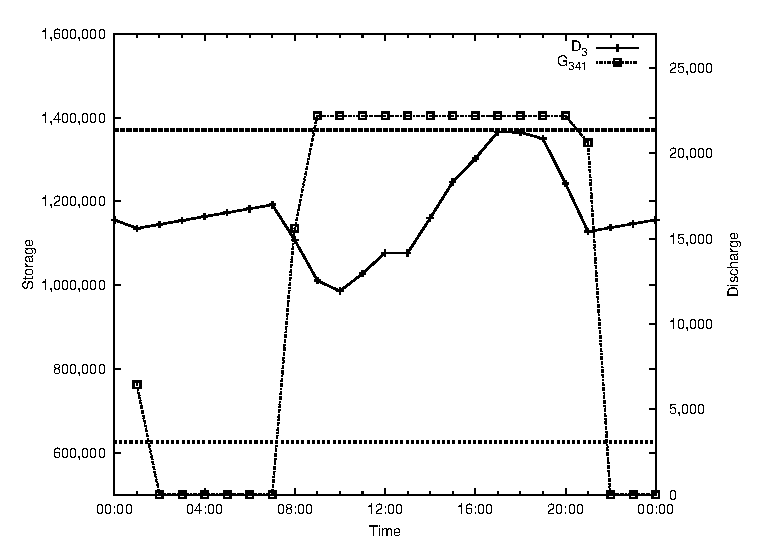
\includegraphics[width=0.9\linewidth]{fig/d3.eps}
  \caption{Storage in $\rm D_{3}$ and Generation Discharge }
  \label{fig:d3}
\end{figure}

\begin{figure}[H]
  \centering
  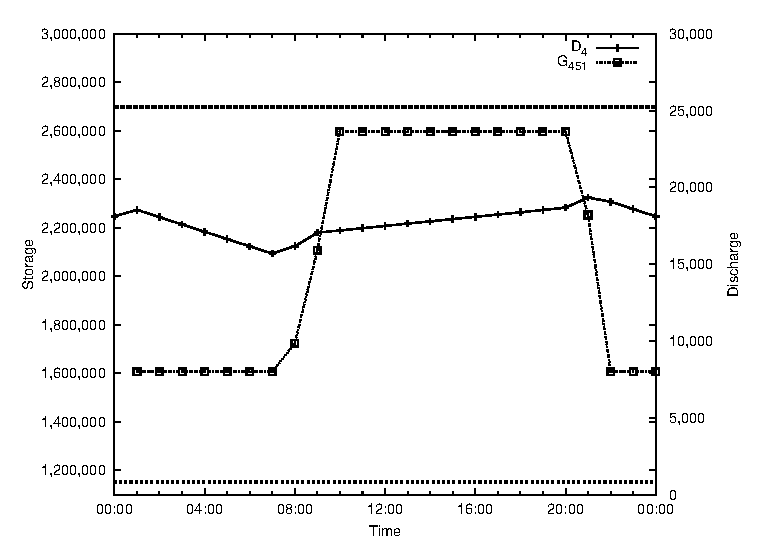
\includegraphics[width=0.9\linewidth]{fig/d4.eps}
  \caption{Storage in $\rm D_{4}$ and Generation Discharge }
  \label{fig:d4}
\end{figure}

\begin{figure}[H]
  \centering
  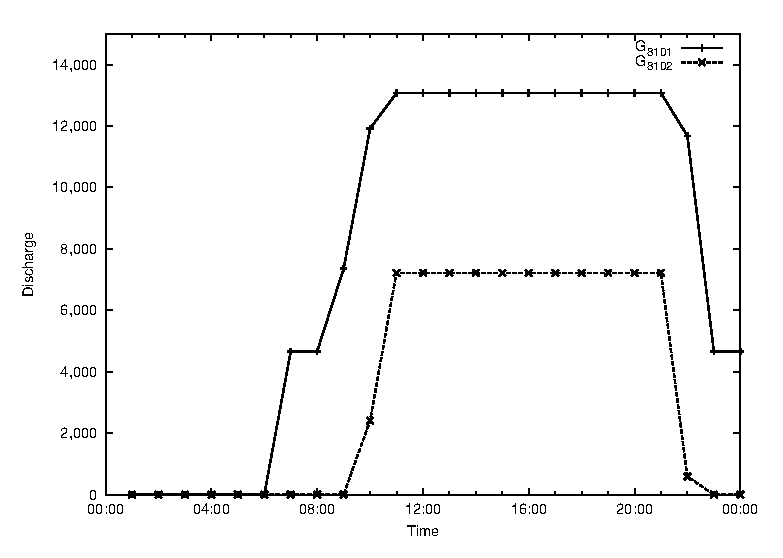
\includegraphics[width=0.9\linewidth]{fig/d8.eps}
  \caption{Discharge from $\rm D_{8}$}
  \label{fig:d8}
\end{figure}

\begin{figure}[H]
  \centering
  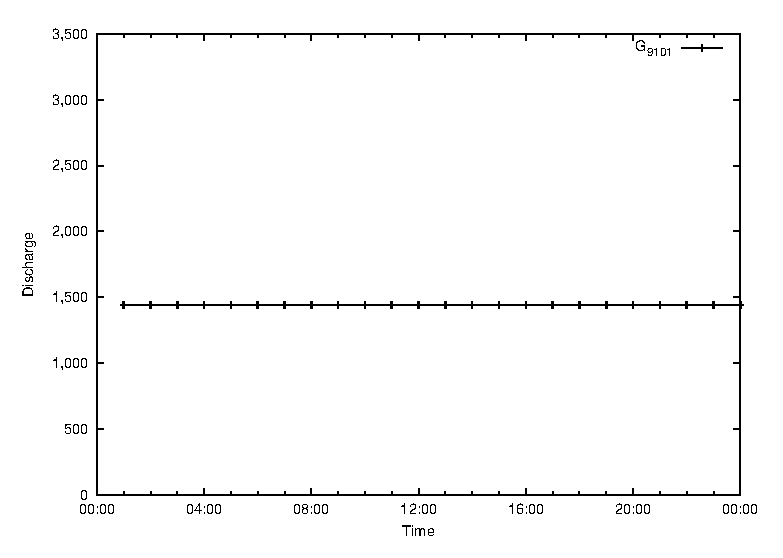
\includegraphics[width=0.9\linewidth]{fig/d9.eps}
  \caption{Discharge from $\rm D_{9}$}
  \label{fig:d9}
\end{figure}

%%%%%%%%%
\section{まとめ}
%%%%%%%%%

本章では,実際の水系に準ずる例題を用いた計算例を示し,%
その結果から提案モデルの妥当性を確認した.
次章では,結論として本研究で得られた成果と今後の課題を要約する.


% 第5章 低速飛行特性
%!TEX root = main.tex

%%%%%%%%%%%%%%%%%%%%%%
\chapter{低速飛行特性}
\label{flight_char}
%%%%%%%%%%%%%%%%%%%%%%

本章では,実験で得られたデータから,これまでに述べた力学モデルを用いてパラメータ同定を行ない,低速飛行時の飛行特性について検証する.まず機体が持つ固有振動をとらえるために,線形モデルによる固有値解析を行なう.次に,同定を行なった結果から,設定した空気力モデルの妥当性を検討する.最後に,同定結果をCFD解析の結果と比較し,考察を行なう.

%%%%%%%%%%%%%%%%%%%%%%%%%%%%%%%%%%%%
\section{線形モデルによる固有値解析}
\label{sec:analyze}
%%%%%%%%%%%%%%%%%%%%%%%%%%%%%%%%%%%%

本節では,線形化された機体の飛行モデルを用いて,固有値解析を行なう.まず,式(\ref{eq:lin_model})より,$\Delta$を省略して微分方程式をまとめると
\begin{equation}
  \dfrac{d}{dt}
  \underbrace{
  \left[
  \begin{array}{cccc}
    u \\
    \alpha \\
    q \\
    \theta \\
  \end{array}
  \right]}_{\underline{x}} =
  \underbrace{
  \left[
  \begin{array}{cccc}
    X_u & X_\alpha & X_q & X_\theta \\
    \overline{Z_u} & \overline{Z_\alpha} & \overline{Z_q} & \overline{Z_\theta} \\
    \overline{M_u} & \overline{M_\alpha} & \overline{M_q} & \overline{M_\theta} \\
    0 & 0 & 1 & 0
  \end{array}
  \right]}_{A}
  \underbrace{
  \left[
  \begin{array}{cccc}
    u \\
    \alpha \\
    q \\
    \theta \\
  \end{array}
  \right]}_{\underline{x}} +
  \underbrace{
  \left[
  \begin{array}{cccc}
    X_{\delta_e} & X_{T_m} & 0 & 0 \\
    \overline{Z_{\delta_e}} & \overline{Z_{T_m}} & \overline{Z_{T_r}} & \overline{Z_{T_f}} \\
    \overline{M_{\delta_e}} & \overline{M_{T_m}} & \overline{M_{T_r}} & \overline{M_{T_f}} \\
    0 & 0 & 0 & 0
  \end{array}
  \right]}_{B}
  \underbrace{
  \left[
  \begin{array}{cccc}
    \delta_e \\
    T_m \\
    T_r \\
    T_f \\
  \end{array}
  \right]}_{\underline{u}}
\end{equation}
となる.プロセスノイズを省略すれば,この状態方程式は行列$A,B$と状態量$\underline{x}$,入力$\underline{u}$を用いることによって
\begin{equation}
  \dfrac{d\underline{x}}{dt} = A\underline{x} + B\underline{u}
\label{eq:matrix_A}
\end{equation}
と表すことができる.したがってこれを連続時間システムとすれば,一般に
\begin{equation}
  \underline{x}(t) = e^{At}\underline{x}(0) + \int_0^t e^{A(t-\tau)}B\underline{u}(\tau) d\tau
  \label{eq:system}
\end{equation}
が得られる.式(\ref{eq:system})の右辺第1項目は,斉次方程式の一般解であり,行列$A$の固有値に従う挙動を示す.右辺第2項目は特殊解であり,入力$\underline{u}$による振動数と行列$A$の固有値に従う挙動を示す.

% ここで入力$\underline{u}$が,振動や減衰を表す関数
% \begin{equation}
%   \underline{u} = \sum \underline{f} e^{\omega t}
% \end{equation}
% であるとする.ただし$\omega$は複素数($\omega \in \mathbb{C}$)である.これにより,状態量$\underline{x}$は解析的に解くことができ
% \begin{equation}
%   \underline{x} = \left(\sum_{i}C_i x_i e^{\lambda_i t}\right) +
%   \sum(\omega I - A)^{-1} \underline{f} e^{\omega t}
% \end{equation}
% となる.ここで右辺第1項は,ある係数$C_i$,行列$A$の固有値$\lambda_i$,固有ベクトル$x_i$で表された一般解で,状態に固有な振動や発散,減衰などを表している.右辺第2項は特殊解であり,入力と同じ周波数成分を持つ.つまり,外乱がない限り,状態量は周波数成分として固有振動数や入力に存在する周波数成分に相関するということである.


そこで,\ref{sec:filter}小節でも述べたように,固有振動数を計算することで機体の運動が持つおおよその周波数帯をつかみ,データのフィルタリングに利用する.実際に式(\ref{eq:matrix_A})の行列$A$について,固有値を計算して絶対値をプロットしたものがFig. \ref{fig:eigenvalue}である.ただし,実験中の風の影響などの外乱が大きいと思われるデータは除き,計算を行なった.行列$A$が4次の正方行列であるため,各データ点ごとに最大4つの固有値を持ち,それぞれ色分けされている.グラフ内の縦線は,複数の実験データそれぞれの境界を示す.

Fig. \ref{fig:eigenvalue}から,機体の回転翼機モードにおける低速飛行縦運動の固有振動数は,おおよそ0〜5$\mathrm{[Hz]}$であることが見て取れる.つまり,この範囲内の周波数はフィルタリングなどの処理で落としてはいけない.

\begin{figure}[H]
	\centering
	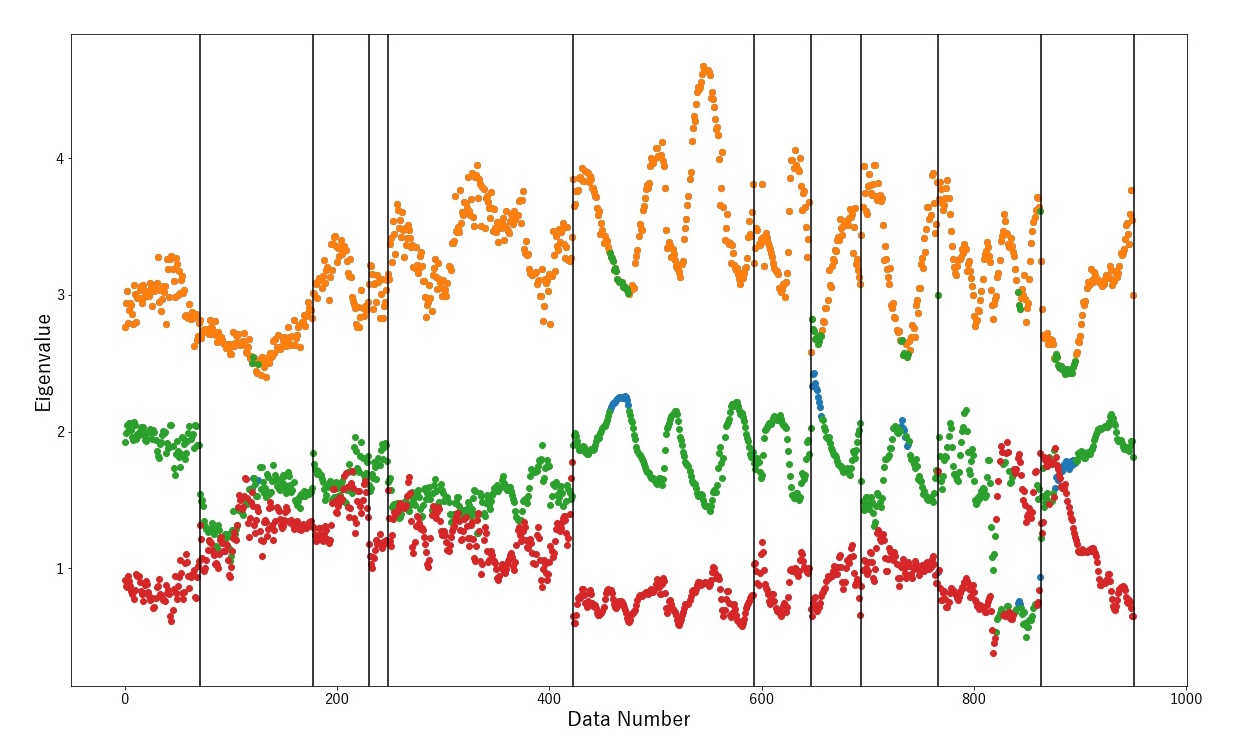
\includegraphics[clip,width=15.0cm,bb=0 0 1250 750]{./z_figure_files/chapter5/1_eigenvalue.jpeg}
	\caption{Absolute value of eigenvalue of matrix A}
	\label{fig:eigenvalue}
\end{figure}

%%%%%%%%%%%%%%%%%%%%%%%%%%%%
\section{空気力モデルの検証}
\label{sec:airf_model_ver}
%%%%%%%%%%%%%%%%%%%%%%%%%%%%

本節では,パラメータ同定の結果から,式(\ref{eq:L})〜(\ref{eq:Ma})で設定した空気力モデルが妥当であるかを考える.Fig. \ref{fig:CL_si}〜\ref{fig:Cm_si}にはそれぞれ3種類の色分けされた点がプロットされている.これらは以下に示す3通りのデータセットをプロットしている.

\begin{itemize}
  \setlength{\leftskip}{1.0cm}
  \setlength{\rightskip}{0.5cm}
  \item[Data1(青)] $L_{log},D_{log},M_{a_{log}}$を用いて,各ステップごとに算出した空力係数群\\(ログデータから得られた,真値に近いと考えられる値)
  \item[Data2(黄)] 式(\ref{eq:L_o})〜(\ref{eq:Ma_o}),すなわち$k_* V_a$の項を除いたモデルを用いて同定した結果から,各ステップごとに算出した空力係数群
  \item[Data3(緑)] 式(\ref{eq:L})〜(\ref{eq:Ma}),すなわち本研究で仮定する空気力モデルを用いて同定した結果から,各ステップごとに算出した空力係数群
\end{itemize}

ただし,式(\ref{eq:CL}),~(\ref{eq:Cm})より空力係数に関係する変数は,$\alpha,\dot{\alpha},q,\delta_e,V_a$の計5個あるが,その中から$V_a$を横軸にとった場合を図示している.

$C_L$は各データセット間でそれほど大きな差は見られないが,$C_D,C_m$においては,Data1が真値に近い値であると考えれば,Data2よりもData3のほうが,よりData1に沿うように点在していることが分かる.

さらに詳細にモデルを評価するための精度評価指標として,平均平方二乗誤差(Root Mean Square Error,RMSE)を用いる.$k$番目のステップにおけるData1の値を実測値として$C_{obs,k}$,比較対象とするデータセットの値を予測値として$C_{pred,k}$とすると
\begin{equation}
  \mbox{RMSE} = \sqrt{\dfrac{1}{N}\sum_{k}(C_{obs,k}-C_{pred,k})^{2}} \quad (N\mbox{:サンプルデータ数})
  \label{eq:rmse}
\end{equation}
となる\cite{}.式(\ref{eq:rmse})を用いて,各空力係数に対して計算した結果をTable \ref{tb:rmse}に示す.結果から,Data2よりもData3のほうが,誤差は小さく予測精度が高いことがわかる.

したがって,回転翼機モードの空気力モデルにおいては,$k_* V_a$の項を含めることが妥当であると考えられる.特に,$C_D$における$k_D V_a$の効果が大きく,この結果は従来研究\cite{}の結果とも整合する.

\begin{table} [htbp]
  \begin{center}
    \caption{Comparing RMSE values}
    \label{tb:rmse}
    \begin{tabular}{|c||c|r|} \hline
      ~ & Data set & RMSE value \\ \hline \hline
      $C_L$ & Data2 & 0.4045 \\
       & Data3 & 0.3443 \\ \hline
       $C_D$ & Data2 & 0.5764 \\
        & Data3 & 0.3883 \\ \hline
        $C_m$ & Data2 & 0.8432 \\
         & Data3 & 0.7419 \\ \hline
    \end{tabular}
  \end{center}
\end{table}

\begin{figure}[htbp]
	\begin{center}
		\begin{tabular}{c}
			\begin{minipage}{0.5\hsize}
				\begin{center}
					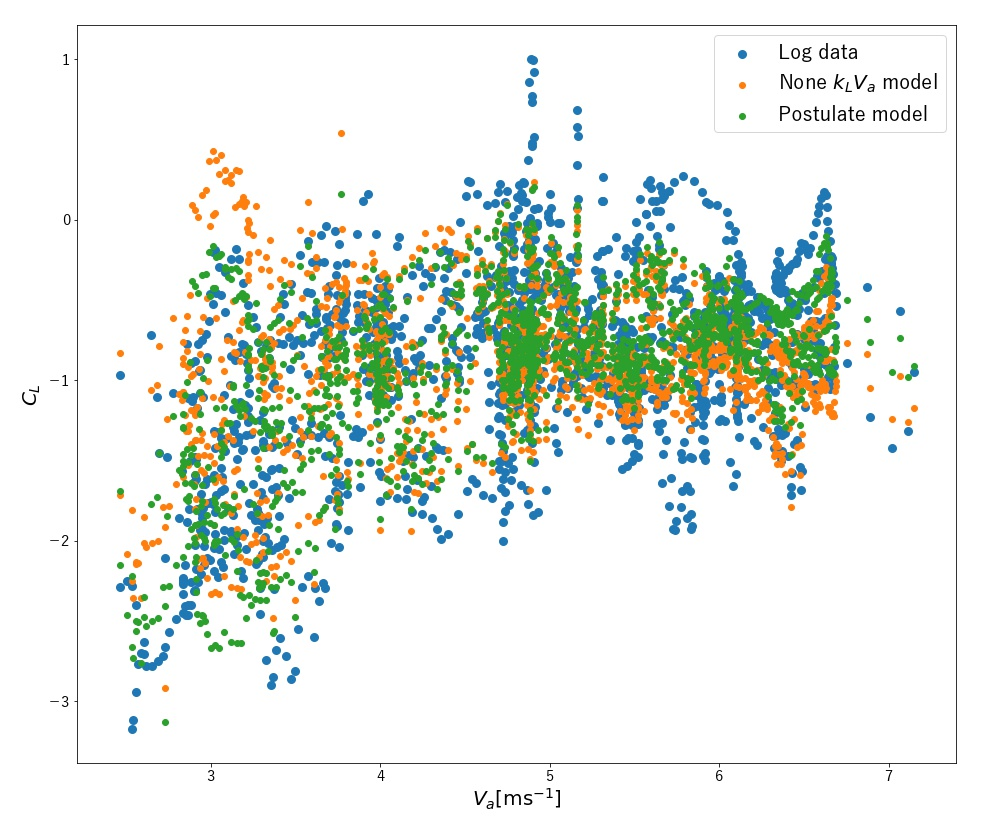
\includegraphics[clip,width=7.5cm,bb=0 0 864 654]{./z_figure_files/chapter5/2_CL.jpeg}
					\caption{$C_L$ plots}
					\label{fig:CL_si}
				\end{center}
			\end{minipage}
			\begin{minipage}{0.5\hsize}
				\begin{center}
					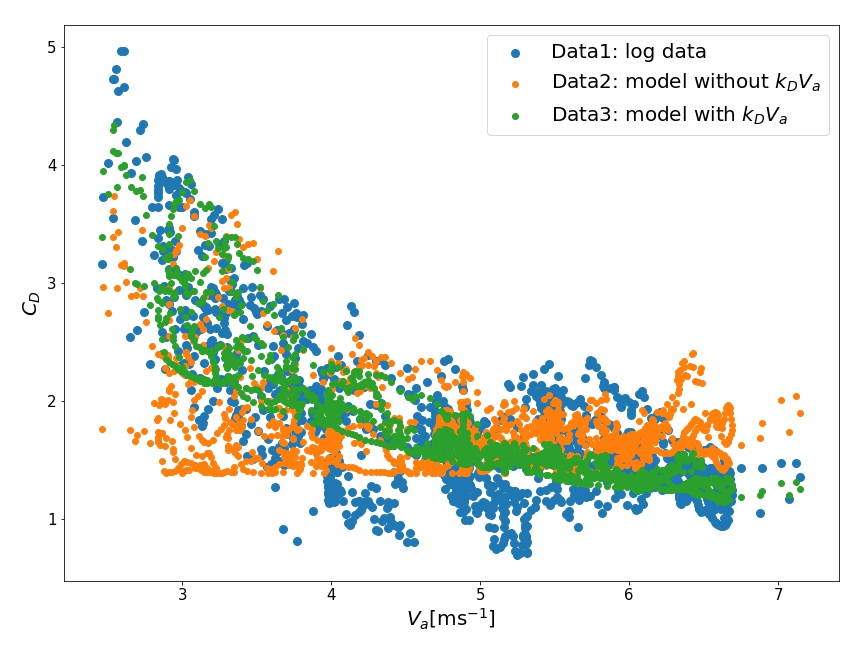
\includegraphics[clip,width=7.5cm,bb=0 0 864 654]{./z_figure_files/chapter5/3_CD.jpeg}
					\caption{$C_D$ plots}
					\label{fig:CD_si}
				\end{center}
			\end{minipage}
		\end{tabular}
	\end{center}
\end{figure}
\begin{figure}[H]
  \begin{center}
    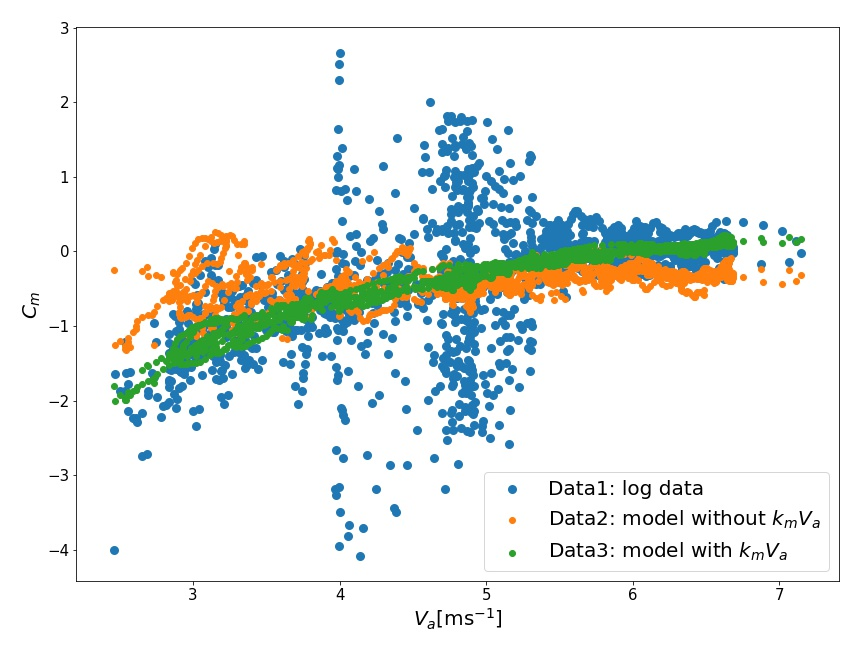
\includegraphics[clip,width=7.5cm,bb=0 0 864 654]{./z_figure_files/chapter5/4_Cm.jpeg}
    \caption{$C_m$ plots}
    \label{fig:Cm_si}
  \end{center}
\end{figure}


%%%%%%%%%%%%%%%%%%%%%%%%%%%%%%%
\section{CFDによる解析結果との比較}
\label{sec:cfd}
%%%%%%%%%%%%%%%%%%%%%%%%%%%%%%%

本節では,パラメータ同定結果の妥当性をさらに検証するために,\cite{kawano}で得られた対気速度$V_a=5\mathrm{[m s^{-1}]}$のCFD解析結果とも比較する.このため,\ref{sec:airf_model_ver}節で示したData2,Data3のデータセットから,$4.5\mathrm{[m s^{-1}]} \leq V_a \leq 5.5\mathrm{[m s^{-1}]}$であるものを選んで比較した.Fig. \ref{fig:cfd_L}〜\ref{fig:cfd_Ma}に,迎角$\alpha$を横軸にとり,揚力・抗力・ピッチモーメントそれぞれの空力係数をプロットしたものを示す.青の点($C_{*_{log}}$)がログデータから算出された値,赤の点($C_{*_{CFD}}$)がCFD解析による値,黄色の点($C_{*_{SI}}$)が同定結果をもとに,CFDに合わせて,$\alpha=-20\mathrm{[deg]},-10\mathrm{[deg]},0\mathrm{[deg]}$の3点において再現された値である.ただし,$C_{*_{CFD}}$と$C_{*_{SI}}$については$\alpha$との関係性を見るために,各点と同じ色で回帰直線を引いてある.

$C_L$について,CFDの解析結果は$\alpha$が大きいほど数値も大きくなることが見て取れる.しかし,ログデータや,特に同定結果を見ると,$\alpha$が$-5\mathrm{[deg]}$付近を境に$\alpha$の上昇に伴って数値が小さくなっていくように見える.CFDでは,ロータは回していない状態で解析を行なっているため,$\alpha$が大きいとき,ロータによって発生する空気の流れによって,負の揚力が発生しているのではないかと考えられる.

次に$C_D$について,同定結果とCFD解析結果がほぼ一致している一方で,ログデータとは一致していない.これは抗力係数のうち,迎角によって変化するとされる有害抵抗係数による影響だと考えられる\cite{katou}.同定に用いる式(\ref{eq:D_o})の設定を見直す必要があると思われる.

最後に$C_m$について,ログデータにはばらつきがあるものの,どの結果も$\alpha$の値によらずほぼ一定の値を取っている.CFDの解析結果が大きく離れているのは,ロータ推力の推算による誤差が大きい可能性が考えられる.ロータ推力の算出方法も改善の余地があると思われる.

\begin{figure}[htbp]
	\centering
		\begin{tabular}{c}
			\begin{minipage}{0.5\hsize}
				\centering
					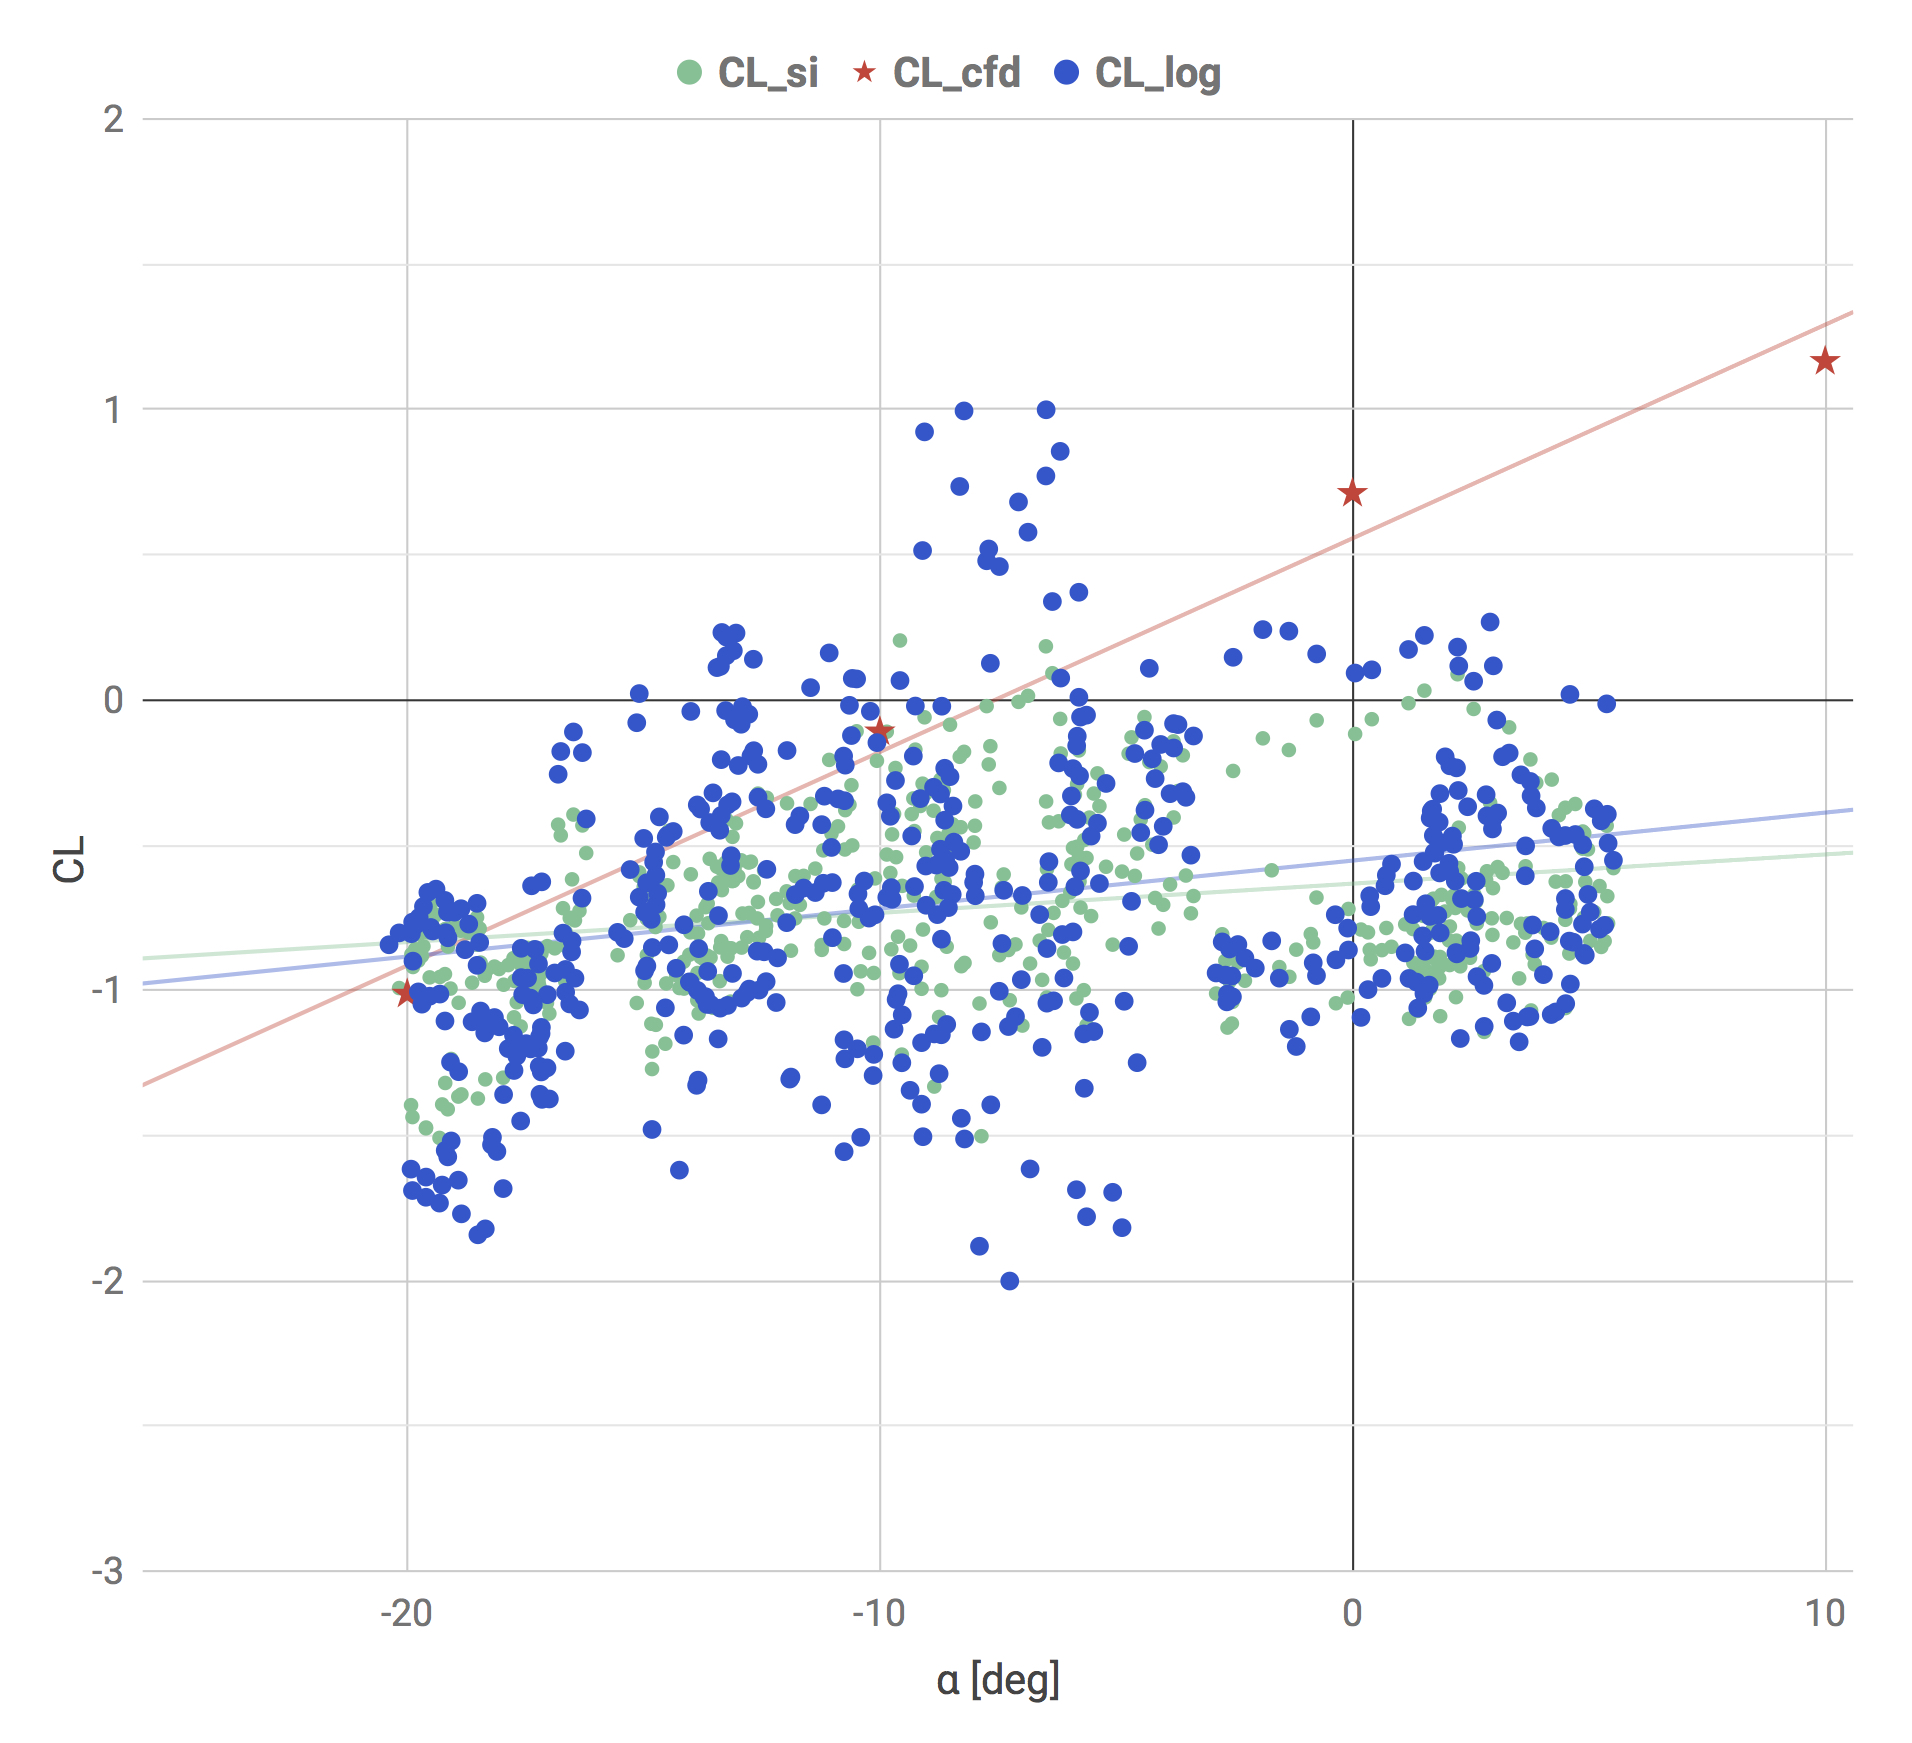
\includegraphics[clip,width=7.5cm,bb=0 0 1912 1743]{./z_figure_files/chapter5/cfd_L.jpeg}
					\caption{\small{Comparing $C_L$ results of CFD and identification}}
					\label{fig:cfd_L}
			\end{minipage}
			\begin{minipage}{0.5\hsize}
				\centering
					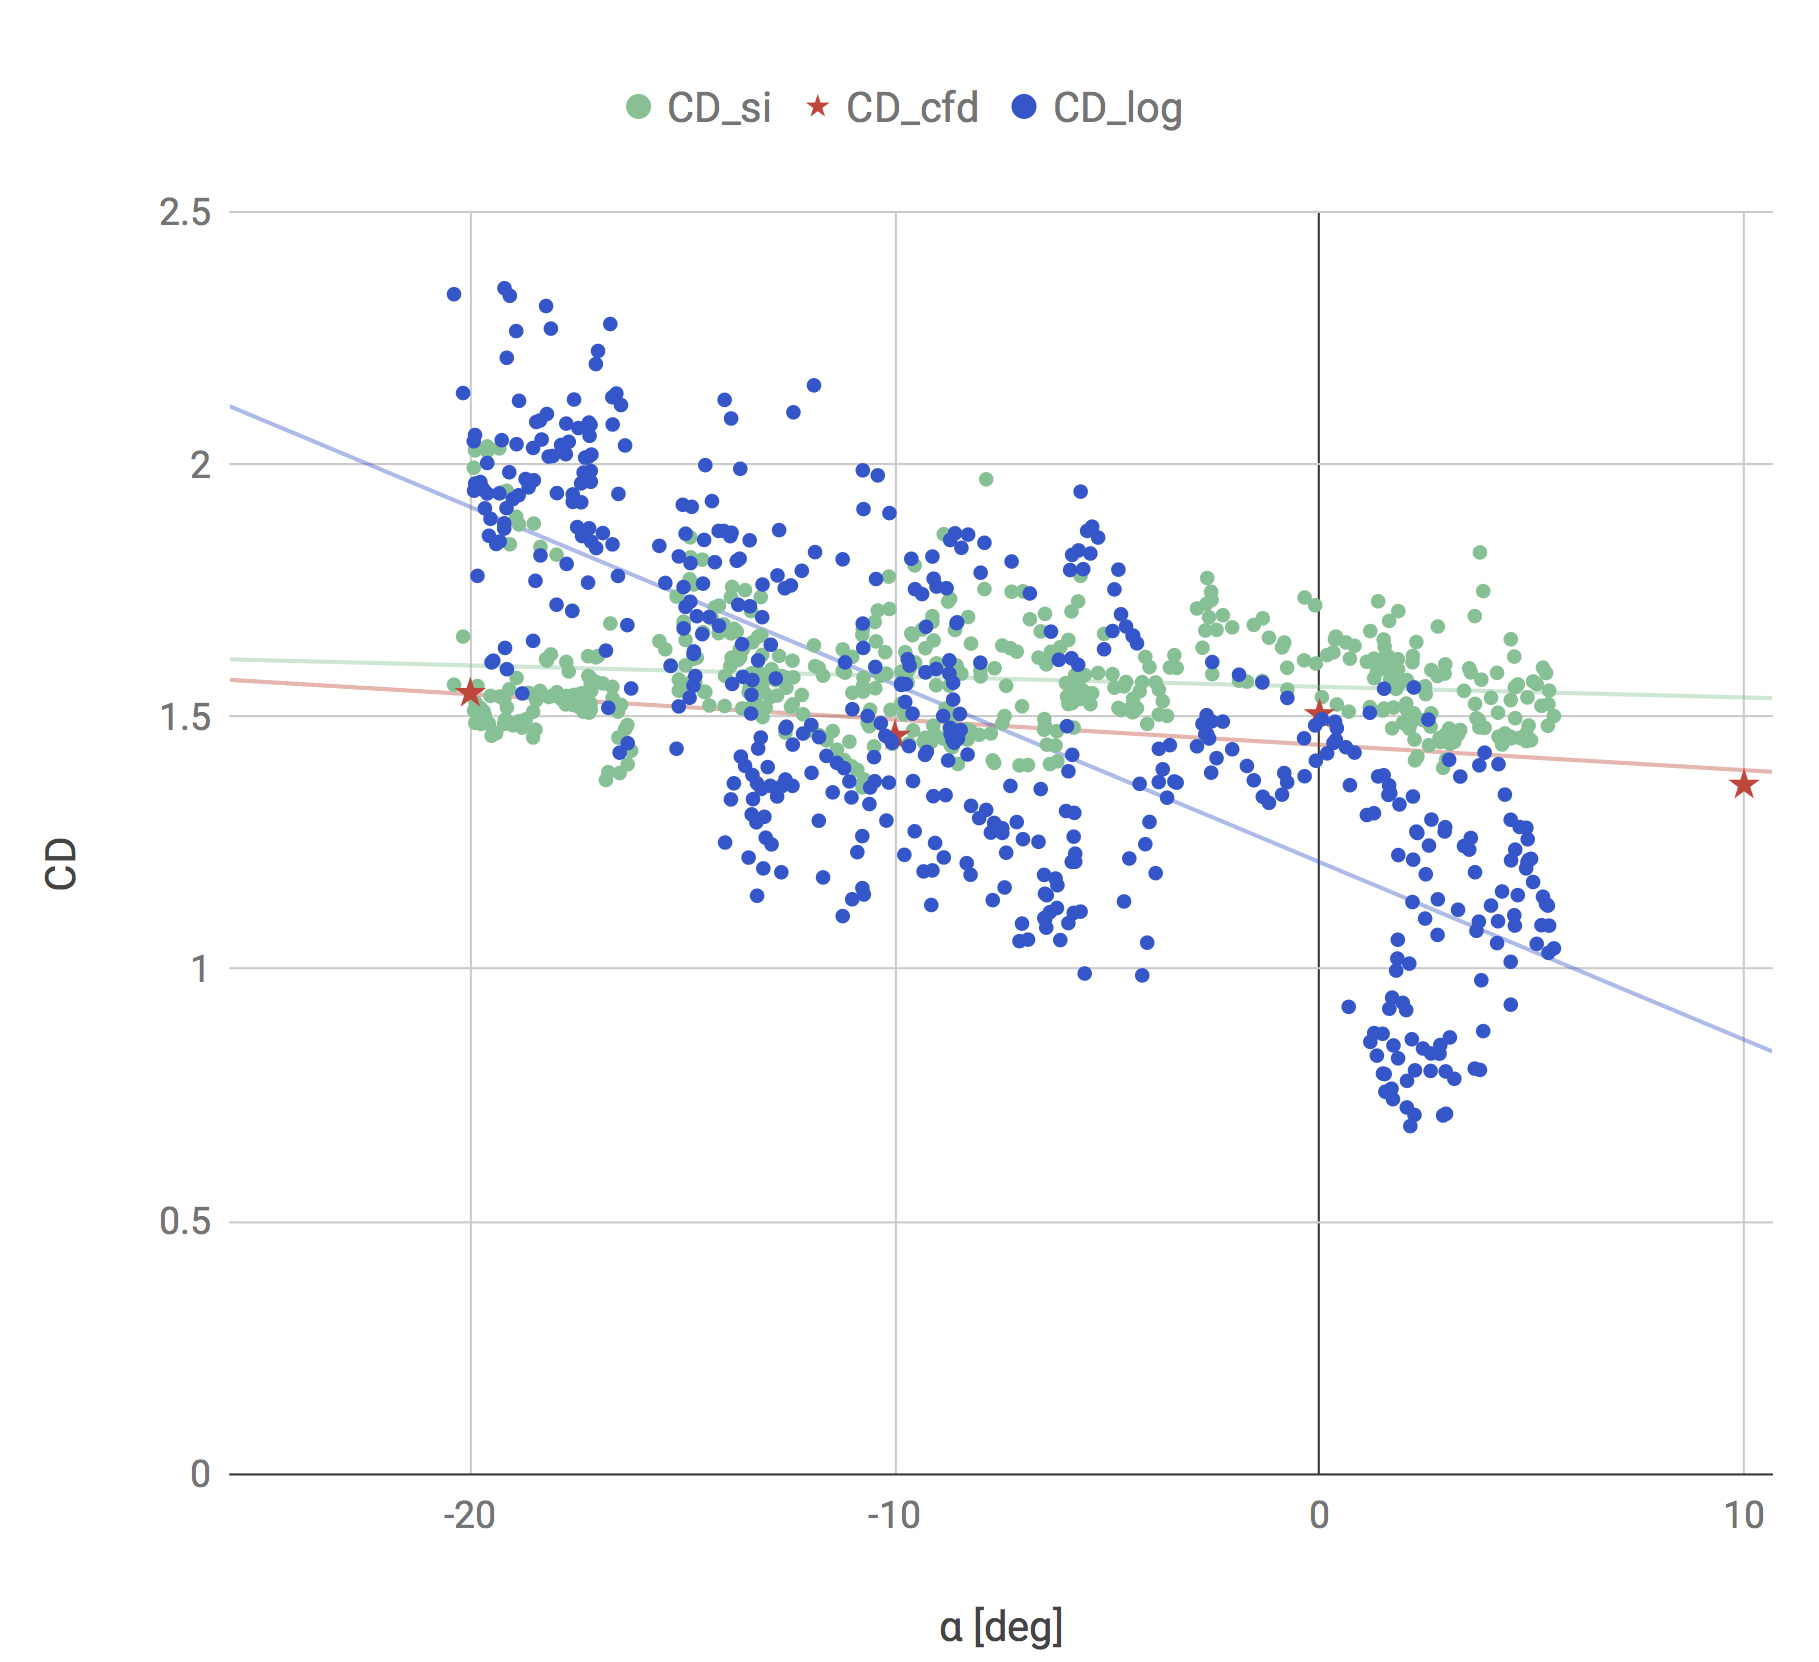
\includegraphics[clip,width=7.5cm,bb=0 0 1819 1662]{./z_figure_files/chapter5/cfd_D.jpeg}
					\caption{\small{Comparing $C_D$ results of CFD and identification}}
					\label{fig:cfd_D}
			\end{minipage}
		\end{tabular}
\end{figure}
\begin{figure}[H]
  \centering
    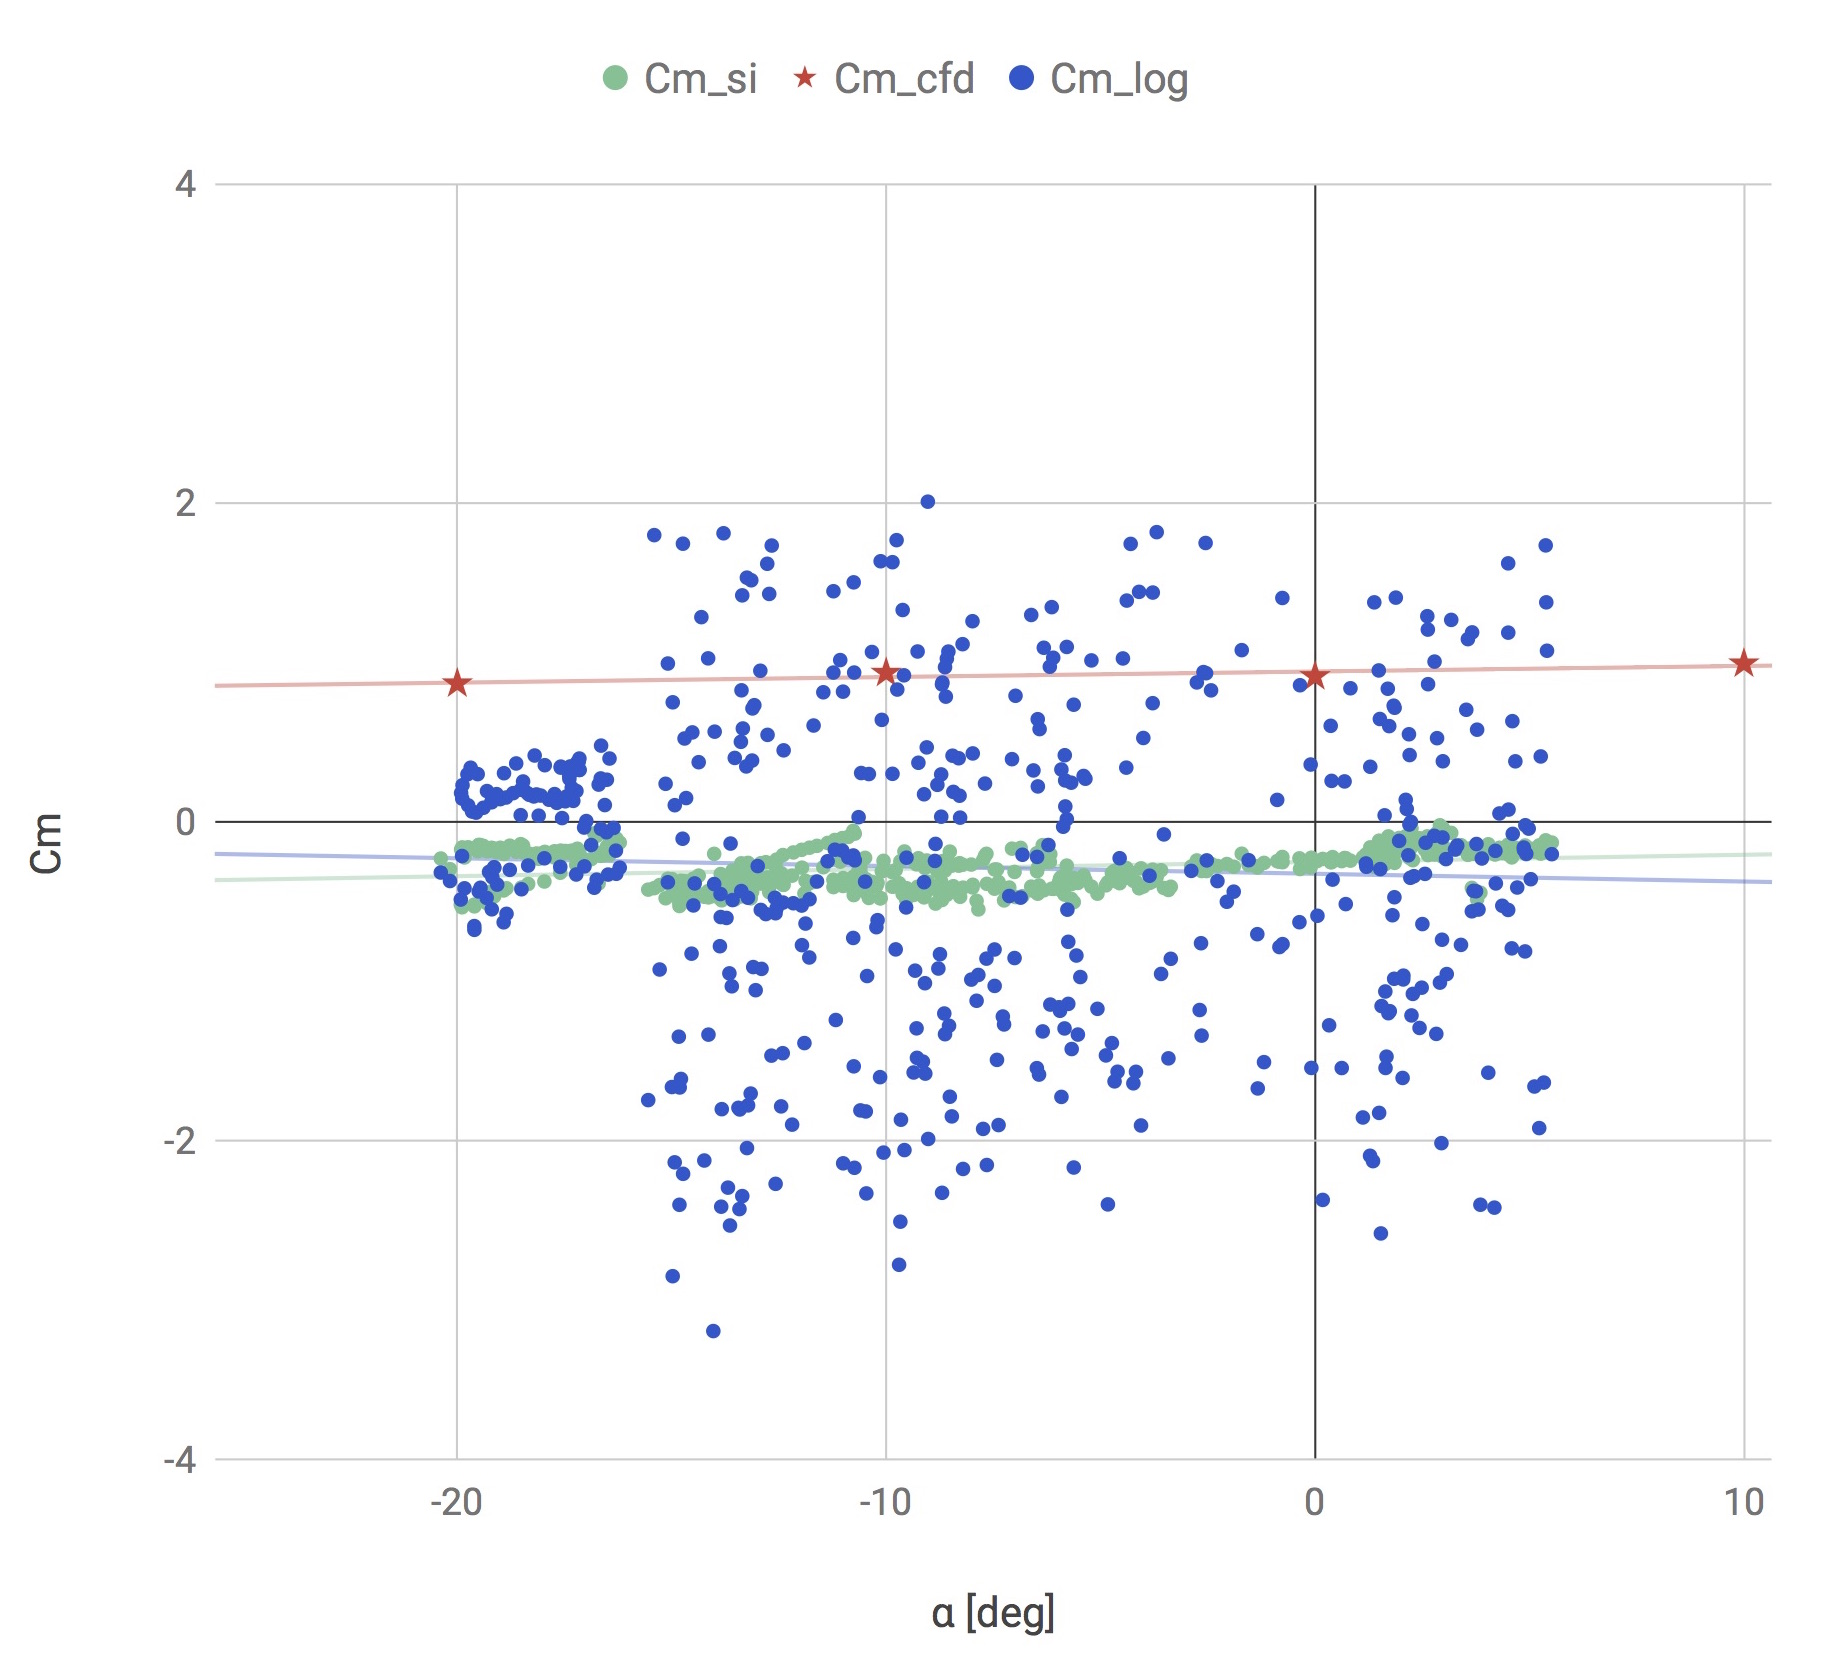
\includegraphics[clip,width=7.5cm,bb=0 0 1832 1662]{./z_figure_files/chapter5/cfd_m.jpeg}
    \caption{\small{Comparing $C_m$ results of CFD and identification}}
    \label{fig:cfd_Ma}
\end{figure}

% 結論
%!TEX root = main.tex

%%%%%%%%%%%%%%
\chapter{結論}
\label{conclusion}
%%%%%%%%%%%%%%

本論文では,開発機体である小型UAVの回転翼機モードを対象とし,パラメータ同定による飛行特性の取得と,飛行特性の解析について述べてきた.結論として,まずは各章ごとに概略をまとめる.
序論では小型UAVが大規模災害発生時に有用であることを示した上で,その中でも固定翼機と回転翼機の両方の長所を兼ね備えたティルトロータ型UAVに着目していることを述べた.加えて,我々が目指す高度な自律飛行のために,飛行特性の取得が重要であること,飛行特性の取得には一般の航空機に用いられているパラメータ同定手法を採用したことなどを述べた.研究対象を明確にするために,第2章では実験に使用した機体について述べた.

第3章では,開発機体の力学モデルを取り扱った.機体を単一の剛体とみなし,6自由度の非線形微分方程式および姿勢角の微分方程式を記述した.さらにそれらを縦方向と横方向の運動に分けて,本研究では縦運動にのみ着目し,飛行モデルを設定した.また,安定微係数による微小擾乱方程式を導出することで飛行モデルの線形化を行なった.一般の航空機とは異なる空気力モデルの設定もここで行なった.

第4章では,実機実験で得られた飛行ログデータを用いたパラメータ同定について述べた.まずデータの前処理として,直接得られないデータの算出方法や,フーリエ変換による周波数領域でのフィルタリング処理について説明した.また,最小二乗法による同定の手法を説明した後,実際の同定結果を示した.

第5章では,第4章で述べたパラメータ同定の結果もふまえ,回転翼機モードにおける低速飛行特性の解析およびモデルの妥当性の検証を行なった.また,CFDの解析結果との比較も行なっている.

\vspace{5pt}

本研究をふまえた上で提唱する今後の課題として,以下のような項目が挙げられる.
\begin{itemize}
  \item[(1)] より多く,より正確なデータの取得
  \item[(2)] 固有値解析における入力項の考慮
  \item[(3)] パラメータ推定手法の検証
  \item[(4)]
\end{itemize}

以上に挙げた項目について一つずつ詳細を述べる.(1)について,第4章でも述べた通り実験データには誤差が含まれている.これを少しでも正確なものにするために,データのフィルタリング処理の精度を高くする必要がある.また直接得られないため,ログデータから算出している値についても,算出方法を確立する必要があると思われる.

(2)について,(1)にも関連するが,より精度の高いフィルタリングを行なうために,式(\ref{eq:system})の入力項による影響をさらに考える必要がある.そのために,\cite{narioka}で用いられているウェーブレット解析による時間周波数情報の活用は有効であると考えられる.


\newpage
\addcontentsline{toc}{chapter}{謝辞}
% 謝辞
%!TEX root = main.tex

\chapter*{謝辞}

本研究を進めるにあたり,丁寧なご指導を賜りました神戸大学大学院~システム情報学研究科~准教授~浦久保孝光先生に深く感謝の意を表します.また,非常に有益な御助言を頂戴致しました同大学院工学研究科~教授~玉置久先生に感謝致します.航空機力学という未知の分野ではありましたが,研究を通して様々な基礎分野を勉強させていただき,実験的に応用するところまで経験させていただきました.研究がいかに有意義なもので,勉学がいかに楽しいものであるか,短い期間ではありましたが,再確認させていただきました.熱心なご指導を頂いたことを重ねて感謝致します.

また共同研究として,佐部浩太郎様,平井真二様,村越象様をはじめとしたエアロセンス株式会社の皆様には,機体の開発にご協力いただきました.特に名前を挙げさせていただきました3名の方々には,実験の際に直接ご助言を頂いたこと,感謝致します.また,双葉電子工業~恩田哲男様,徳島大学~准教授~三輪昌史先生には,データ取得のための飛行実験の際に,パイロットとしてご協力いただきました.本当にありがとうございました.

そして,研究だけでなく,日々の生活においてもお世話になった同研究室の皆様にも深く感謝致します.加えて,私を様々な面で支えてくれた友人の皆様,そして何よりも私の大学生活を支えてくださった両親には感謝してもしきれません.

私が大学生活で関わったすべての皆様に,ここで改めて深く感謝申し上げます.

\newpage
%%%%謝辞
\addcontentsline{toc}{chapter}{参考文献}
% 参考文献
%!TEX root = main.tex

\begin{thebibliography}{99}

%\bibitem{ラベル} 著者: タイトル, 編集社, ページ (年)
% \bibitem{}
%  : ``'' , no. , pp.  ()

\bibitem{shimada}
嶋田有三,佐々修一 : ``飛行力学'', 森北出版株式会社 , pp.26-28 (2017)
\bibitem{katayanagi}
片柳亮二 : ``航空機の飛行力学と制御'', 森北出版株式会社 , pp.4-17 (2007)
\bibitem{yoshimura}
吉村啓史 : ``強風下におけるティルトロータ型UAVのホバリング飛行'', 神戸大学大学院システム情報学研究科修士論文 , pp.9-12 (2018)
\bibitem{etkin}
Bernard Etkin,Lloyd Duff Reid : ``\textit{Dynamics of FLIGHT}'', John Wiley & Sons. Inc. , pp.18-92 (1959)
\bibitem{yamana}
山名正夫 : ``VTOLとSTOL'', 日本航空学会誌 , 9巻91号 , pp.255-269 (1961)
\bibitem{katou}
加藤寛一郎,大屋昭男,柄沢研治 : ``航空機力学入門'', 東京大学出版会(1982)
\bibitem{oota}
太田有三 : ``現代制御'', 株式会社オーム社 , pp.42-55 (2014)
\bibitem{kawata}
川田昌克 : ``MATLAB/Simulinkと実機で学ぶ制御工学 ―PID制御から現代制御まで―'', TechShare (2013)
\bibitem{yoshikawa}
吉川友真 : ``ティルトロータ型UAVの固定翼機モードにおける飛行特性'', 神戸大学大学院システム情報学研究科修士論文 , pp.24-25 (2018)
\bibitem{klein}
Eugene A.Morelli,Vladislav Klein : ``Aircraft System Identification Theory and Practice Second Edition'', Sunflyte Enterprises (2016)
\bibitem{eugene}
Eugene A.Morelli : ``Practical Aspects of the Equation-Error Method for Aircraft Parameter Estimation'', NASA Langley Research Center , pp.1-5 (2006)
\bibitem{narioka}
成岡優 : ``システム同定による小型無人航空機の飛行特性の取得'', 東京大学大学院工学系研究科博士論文 , pp.117-142 (2016)

\end{thebibliography}

\newpage
%%%参考文献
\addtocontents{toc}{\protect\contentsline {chapter}{付録}{}}
\appendix
% \pagestyle{empty}
% \textheight=24cm
% \addtocounter{chapter}{1}
% \noindent
% {\Large \bf 付録}\\
%
% \noindent
%
% 付録です.
%%%%付録
\end{document}%%%%%%%%%%%ドキュメントの終了
